% This template was downloaded from:
% http://www.LaTeXTemplates.com
%
% Version 2.x major modifications by:
% Vel (vel@latextemplates.com)
%
% This template is based on a template by:
% Steve Gunn (http://users.ecs.soton.ac.uk/srg/softwaretools/document/templates/)
% Sunil Patel (http://www.sunilpatel.co.uk/thesis-template/)
%
% Template license:
% CC BY-NC-SA 3.0 (http://creativecommons.org/licenses/by-nc-sa/3.0/)
%
%%%%%%%%%%%%%%%%%%%%%%%%%%%%%%%%%%%%%%%%%


%----------------------------------------------------------------------------------------
%	PACKAGES AND OTHER DOCUMENT CONFIGURATIONS
%----------------------------------------------------------------------------------------

\documentclass[
11pt, % The default document font size, options: 10pt, 11pt, 12pt
%oneside, % Two side (alternating margins) for binding by default, uncomment to switch to one side
% serbian, % ngerman for German
serbian,
singlespacing, % Single line spacing, alternatives: onehalfspacing or doublespacing
%draft, % Uncomment to enable draft mode (no pictures, no links, overfull hboxes indicated)
%nolistspacing, % If the document is onehalfspacing or doublespacing, uncomment this to set spacing in lists to single
%liststotoc, % Uncomment to add the list of figures/tables/etc to the table of contents
%toctotoc, % Uncomment to add the main table of contents to the table of contents
%parskip, % Uncomment to add space between paragraphs
% nohyperref, % Uncomment to not load the hyperref package
headsepline, % Uncomment to get a line under the header
%chapterinoneline, % Uncomment to place the chapter title next to the number on one line
%consistentlayout, % Uncomment to change the layout of the declaration, abstract and acknowledgements pages to match the default layout
]{MastersDoctoralThesis} % The class file specifying the document structure

\usepackage[utf8]{inputenc} % Required for inputting international characters
\usepackage[T1]{fontenc} % Output font encoding for international characters

%\usepackage{mathpazo} % Use the Palatino font by default
\usepackage{amsmath}
% dužine

\usepackage{float}
\usepackage{listings}                                                          
\usepackage{color}

\definecolor{mygreen}{rgb}{0,0.6,0}
\definecolor{mygray}{rgb}{0.5,0.5,0.5}
\definecolor{mymauve}{rgb}{0.58,0,0.82}

                                                                                

% \usepackage[backend=bibtex,style=authoryear,natbib=true]{biblatex} % Use the bibtex backend with the authoryear citation style (which resembles APA)
\usepackage[
  backend=bibtex
  , natbib=true
  , citestyle=numeric
  , bibstyle=numeric
  , sorting=none
  , maxbibnames=99
]{biblatex} % Use the bibtex backend with the authoryear citation style (which resembles APA)


\addbibresource{bib/main.bib} % The filename of the bibliography


% \usepackage[autostyle=true]{csquotes} % Required to generate language-dependent quotes in the bibliography

%----------------------------------------------------------------------------------------
%	MARGIN SETTINGS
%----------------------------------------------------------------------------------------

\geometry{
	paper=a4paper, % Change to letterpaper for US letter
	% inner=3.15cm, % Inner margin
	% outer=3.15cm, % Outer margin
	% bindingoffset=0cm, % Binding offset
	inner=2.5cm, % Inner margin
	outer=3.8cm, % Outer margin
	bindingoffset=.5cm, % Binding offset
	top=1.5cm, % Top margin
	bottom=1.5cm, % Bottom margin
  % showframe, % Uncomment to show how the type block is set on the page
}

%----------------------------------------------------------------------------------------
%	THESIS INFORMATION
%----------------------------------------------------------------------------------------

\thesistitle{Predviđanje funkcija proteina metodama binarne klasifikacije} % Your thesis title, this is used in the title and abstract, print it elsewhere with \ttitle

\supervisor{dr Jovana \textsc{Kovačević}} % Your supervisor's name, this is used in the title page, print it elsewhere with \supname
\examiner{} % Your examiner's name, this is not currently used anywhere in the template, print it elsewhere with \examname
\degree{Informatičar} % Your degree name, this is used in the title page and abstract, print it elsewhere with \degreename
\author{Anja \textsc{Bukurov}} % Your name, this is used in the title page and abstract, print it elsewhere with \authorname
\addresses{https://poincare.matf.bg.ac.rs/~anja\_bukurov/} % Your address, this is not currently used anywhere in the template, print it elsewhere with \addressname

\subject{Bioinformatika} % Your subject area, this is not currently used anywhere in the template, print it elsewhere with \subjectname
\keywords{.} % Keywords for your thesis, this is not currently used anywhere in the template, print it elsewhere with \keywordnames
\university{\href{http://www.bg.ac.rs}{Univerzitet u Beogradu}} % Your university's name and URL, this is used in the title page and abstract, print it elsewhere with \univname
\department{\href{http://www.racunarstvo.matf.bg.ac.rs/}{Katedra za Računarstvo i informatiku}} % Your department's name and URL, this is used in the title page and abstract, print it elsewhere with \deptname
\group{.} % Your research group's name and URL, this is used in the title page, print it elsewhere with \groupname
% \group{\href{http://researchgroup.university.com}{Research Group Name}} % Your research group's name and URL, this is used in the title page, print it elsewhere with \groupname
\faculty{\href{http://matf.bg.ac.rs}{Matematički fakultet}} % Your faculty's name and URL, this is used in the title page and abstract, print it elsewhere with \facname


\AtBeginDocument{
\hypersetup{pdftitle=\ttitle} % Set the PDF's title to your title
\hypersetup{pdfauthor=\authorname} % Set the PDF's author to your name
\hypersetup{pdfkeywords=\keywordnames} % Set the PDF's keywords to your keywords
}
%---------------------------------------------------------------------

\begin{document}

\frontmatter % Use roman page numbering style (i, ii, iii, iv...) for the pre-content pages

\pagestyle{plain} % Default to the plain heading style until the thesis style is called for the body content

%----------------------------------------------------------------------------------------
%	TITLE PAGE
%----------------------------------------------------------------------------------------

\begin{titlepage}
\begin{center}

\vspace*{0.06\textheight}
{\scshape\LARGE \univname\par} % University name
{\scshape\LARGE \facname\par} % University name
\vspace{1.5cm}
\textsc{\Large Master Rad}\\[0.5cm] % Thesis type

\HRule \\[0.4cm] % Horizontal line
{\huge \bfseries \ttitle\par}\vspace{0.4cm} % Thesis title
\HRule \\[1.5cm] % Horizontal line
 
\begin{minipage}[t]{0.4\textwidth}
\begin{flushleft} \large
\emph{Autor:}\\
\href{http://poincare.matf.bg.ac.rs/~anja\_bukurov/}{\authorname} % Author name - remove the \href bracket to remove the link
\end{flushleft}
\end{minipage}
\begin{minipage}[t]{0.4\textwidth}
\begin{flushright} \large
\emph{Mentor:} \\
\href{http://poincare.matf.bg.ac.rs/~jovana/}{\supname} % Supervisor name - remove the \href bracket to remove the link  
\end{flushright}
\end{minipage}\\[2cm]
 
\vfill

% \large \textit{A thesis submitted in fulfillment of the requirements\\ for the degree of \degreename}\\[0.3cm] % University requirement text
% \textit{in the}\\[0.4cm]
% \groupname\\\deptname\\[2cm] % Research group name and department name

{\scshape\LARGE Članovi komsije:\par}\vspace{0.2cm} % University name
dr Jovana Kovačević \\
prof. dr Gordana Pavlović-Lažetić  \\
dr Mladen Nikolić \\

 
\vfill

\vspace{1cm}
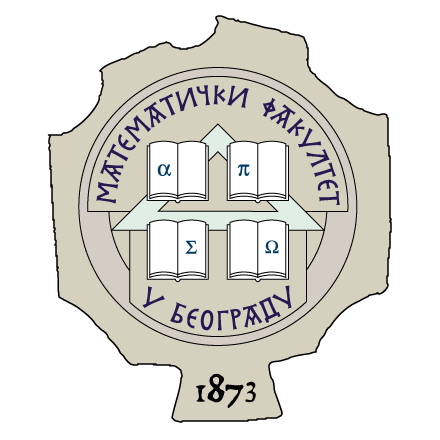
\includegraphics[scale=0.25]{Logo}\\ % University/department logo - uncomment to place it
\vspace{0.5cm}
{\large Beograd, 2019}\\ % Date
 
\vfill
\end{center}
\end{titlepage}


%----------------------------------------------------------------------------------------
%	DECLARATION PAGE
%----------------------------------------------------------------------------------------

% \begin{declaration}
% \addchaptertocentry{\authorshipname} % Add the declaration to the table of contents
% \noindent I, \authorname, declare that this thesis titled, \enquote{\ttitle} and the work presented in it are my own. I confirm that:
%
% \begin{itemize} 
% \item This work was done wholly or mainly while in candidature for a research degree at this University.
% \item Where any part of this thesis has previously been submitted for a degree or any other qualification at this University or any other institution, this has been clearly stated.
% \item Where I have consulted the published work of others, this is always clearly attributed.
% \item Where I have quoted from the work of others, the source is always given. With the exception of such quotations, this thesis is entirely my own work.
% \item I have acknowledged all main sources of help.
% \item Where the thesis is based on work done by myself jointly with others, I have made clear exactly what was done by others and what I have contributed myself.\\
% \end{itemize}
%  
% \noindent Signed:\\
% \rule[0.5em]{25em}{0.5pt} % This prints a line for the signature
%  
% \noindent Date:\\
% \rule[0.5em]{25em}{0.5pt} % This prints a line to write the date
% \end{declaration}
%
% \cleardoublepage

%----------------------------------------------------------------------------------------
%	QUOTATION PAGE
%----------------------------------------------------------------------------------------

% \vspace*{0.2\textheight}
%
% \noindent\enquote{\itshape Thanks to my solid academic training, today I can write hundreds of words on virtually any topic without possessing a shred of information, which is how I got a good job in journalism.}\bigbreak
%
% \hfill Dave Barry

%----------------------------------------------------------------------------------------
%	ABSTRACT PAGE
%----------------------------------------------------------------------------------------

\newcommand{\en}[1]{(engl. \textit{#1})}
\newcommand{\lat}[1]{(latin. \textit{#1})}
\newcommand{\keyword}[1]{\textbf{#1}}
\newcommand{\ikeyword}[1]{\textit{\textbf{#1}}}
\newcommand{\tabhead}[1]{\textbf{#1}}
\newcommand{\code}[1]{\texttt{#1}}
\newcommand{\file}[1]{\texttt{\bfseries#1}}
\newcommand{\option}[1]{\texttt{\itshape#1}}

\newtheorem{definicija}{Definicija}

\iffalse 
\begin{abstract}
\addchaptertocentry{\abstractname} % Add the abstract to the table of contents
% The Thesis Abstract is written here (and usually kept to just this page). The page is kept centered vertically so can expand into the blank space above the title too

\ldots



\end{abstract}

%----------------------------------------------------------------------------------------
%	ACKNOWLEDGEMENTS
%----------------------------------------------------------------------------------------

\begin{acknowledgements}
\addchaptertocentry{\acknowledgementname} % Add the acknowledgements to the table of contents


\end{acknowledgements}
\fi 
%
%----------------------------------------------------------------------------------------
%	LIST OF KEYWORDS
%----------------------------------------------------------------------------------------




%----------------------------------------------------------------------------------------
%	LIST OF CONTENTS/FIGURES/TABLES PAGES
%----------------------------------------------------------------------------------------

\tableofcontents % Prints the main table of contents

%\listoffigures % Prints the list of figures

%\listoftables % Prints the list of tables

%----------------------------------------------------------------------------------------
%	ABBREVIATIONS
%----------------------------------------------------------------------------------------

% \begin{abbreviations}{ll} % Include a list of abbreviations (a table of two columns)
%
% \textbf{LAH} & \textbf{L}ist \textbf{A}bbreviations \textbf{H}ere\\
% \textbf{WSF} & \textbf{W}hat (it) \textbf{S}tands \textbf{F}or\\
%
% \end{abbreviations}

%----------------------------------------------------------------------------------------
%	PHYSICAL CONSTANTS/OTHER DEFINITIONS
%----------------------------------------------------------------------------------------

% \begin{constants}{lr@{${}={}$}l} % The list of physical constants is a three column table
%
% % The \SI{}{} command is provided by the siunitx package, see its documentation for instructions on how to use it
%
% Speed of Light & $c_{0}$ & \SI{2.99792458e8}{\meter\per\second} (exact)\\
% %Constant Name & $Symbol$ & $Constant Value$ with units\\
%
% \end{constants}

%----------------------------------------------------------------------------------------
%	SYMBOLS
%----------------------------------------------------------------------------------------

% \begin{symbols}{lll} % Include a list of Symbols (a three column table)
%
% $a$ & distance & \si{\meter} \\
% $P$ & power & \si{\watt} (\si{\joule\per\second}) \\
% %Symbol & Name & Unit \\
%
% \addlinespace % Gap to separate the Roman symbols from the Greek
%
% $\omega$ & angular frequency & \si{\radian} \\
%
% \end{symbols}

%----------------------------------------------------------------------------------------
%	DEDICATION
%----------------------------------------------------------------------------------------

%\dedicatory{} 

%----------------------------------------------------------------------------------------
%	THESIS CONTENT - CHAPTERS
%----------------------------------------------------------------------------------------

\mainmatter % Begin numeric (1,2,3...) page numbering

\pagestyle{thesis} % Return the page headers back to the "thesis" style



% Include the chapters of the thesis as separate files from the Chapters folder
% Uncomment the lines as you write the chapters

\chapter{Uvod} % Main chapter title
\label{Chapter1}

%  Lee2007...
%a0236.....
%bti1007
% jk i radivojac
Predviđanje funkcije proteina je jedan od najbitnijih zadataka bioinformatike koji može pomoći u velikom broju bioloških problema. Poznavanje funkcije proteina daje nam informacije o njegovim ulogama u organizmu. Metode za eksperimentalno određivanje funkcije proteina su spore u odnosu na brzinu sekvencioniranja genoma koje uvećava broj novih sekvenci. Mnoge metode predviđanja funkcije proteina zasnivaju se na poređenju sekvenci ili struktura proteina za koje je utvrđena funkcija sa onim proteinima za koje je funkcija nepoznata. 

U ovom radu prikazan je razvoj alata za predviđanje funkcije proteina na osnovu njihove primarne strukture. Korišćene su metode binarne klasifikacije i to: metod potpornih vektora, logistička regresija i slučajne šume. Alat je razvijan u programskom jeziku Python.

U poglavlju \ref{Chapter2} uvedeni su biološki pojmovi neophodni za razumevanje rada. U poglavlju \ref{Chapter3} prikazan je način predstavljanja bioloških podataka u računaru, a onda su ukratko predstavljene metode binarne klasifikacije korišćene za razvoj prediktora. Zatim, u poglavlju \ref{Chapter5}, analizirani su podaci o proteinima i njihovim funkcijama, nakon čega je opisana  implementacija alata za predviđanje funkcije proteina. Na kraju, u poglavlju \ref{Chapter6} sumirani su rezultati koje su prediktori dali na izdvojenom skupu proteina za testiranje.
\chapter{Proteini} % Main chapter title
\label{Chapter2}

Sva živa bića sastoje se iz ćelija. U ćelijama se neprestano odvijaju različiti procesi u kojima učestvuju nukleinske kiseline (dezoksiribonukleinka kiselina - DNK i ribonukleinska kiselina - RNK) i proteini. Unutar molekula DNK šifrovan je genetski materijal koji sadrži uputstva za sintezu proteina. 

Proteini su makromolekuli koji igraju mnoge kritične uloge u organizmu. Sačinjavaju više od 50\% suvog dela ćelije i važni su za njenu izgradnju i funkcionisanje. Kontrakcija mišića, strukturna podrška, ubrzavanje i usporavanje hemijskih reakcija, odbrana od virusa i bakterija samo su neke od mnogobrojnih uloga koje proteini obavljaju \cite{radivojac, doktJK}.


\section{Sinteza proteina}

DNK sadrži informacije koje su neophodne ćeliji za izgradnju veoma važnog tipa molekula - proteina. Proteini se sintetišu prilikom genske ekspresije i to u dva koraka: transkripcija i translacija (slika \ref{fig:synthesis}).  Prvi korak je dekodiranje genske poruke, prilikom čega se od DNK sekvence dobija RNK sekvenca. U sastav obe nukleinske kiseline ulazi 4 nukleotida i oni su prikazane u tabeli \ref{tab: nucleotides}. S obzirom da su tri nukleotidne baze iste, proces transkripcije sastoji se iz zamene svakog molekula T molekulom U. 


\begin{figure}[h]
	\centering
	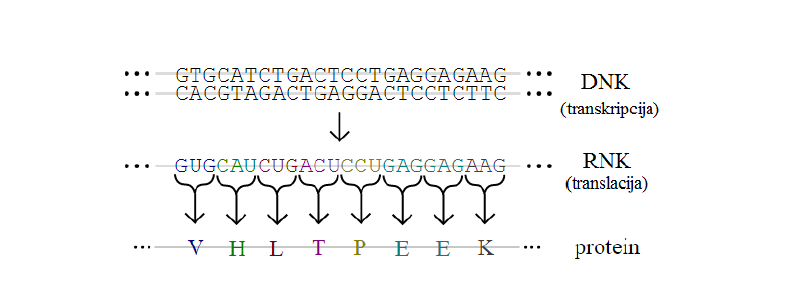
\includegraphics[width=\textwidth]{Figures/protein_synthesis.png}
	\caption{Prikaz procesa sinteze proteina \cite{doktJK}.}
	\label{fig:synthesis}
\end{figure}


\begin{table}[H]
	\centering
	\begin{tabular}{|c|c|c|c|c|}
		\hline
		DNK & adeinin (A) & guanin (G) & citozin (C) & timin (T) \\
		\hline
		RNK & adeinin (A) & guanin (G) & citozin (C) & uracil (U) \\
		\hline             
	\end{tabular}
	\caption{Prikaz nukleinskih kiselina sa nukeotidima koji ih grade.}
	\label{tab: nucleotides}
\end{table}


Sledeći korak, proces translacije, jeste grupisanje aminokiselina kako bi se dobio protein. Genetski kod se čita u grupama od 3 nukleotida koje nazivamo \textit{kodoni}. Svaki kodon odgovara tačno jednoj aminokiselini ili služi da označi kraj sekvence (stop kodon). Na primer, kodon \textbf{GUA} kodira aminokiselinu valin, dok kodon \textbf{UAG} označava kraj sekvence. Na slici \ref{fig:codons} je dat šematski prikaz svih kodona i odgovarajućih aminokiselina. Jedan po jedan, kodoni se prevode u odgovarajuće aminokiseline čime se dobija sekvenca aminokiselina koja čini protein \cite{BMBG, synthesisOnl}.

\begin{figure}[h]
	\centering
	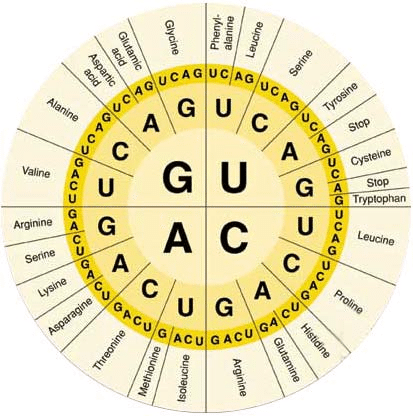
\includegraphics[width=0.8\textwidth]{Figures/codons_chart.png}
	\caption{Prikaz kodona i odgovarajućih aminokiselina.}
	\label{fig:codons}
\end{figure}


\section{Aminokiseline}

Aminokiseline su organska jedinjenja koja se sastoje od karboksilne grupe ($COOH$), aminogrupe ($NH_2$) i bočnog lanca (R-grupa) koji je vezan za $\alpha$-ugljenikov atom i karakterističan je za svaku aminokiselinu. Postoji 20 standardnih aminokiselina i one su prikazane u tabeli \ref{tab: aminoacids}. Pod standardnim aminokiselinama podrazumevaju se one aminokiseline za koje postoji najmanje jedan specifičan kodon u genetskom kodu \cite{biochemestry5, biohUdz, straus}.


\begin{table}
	\centering
	\begin{tabular}{|lcc|lcc|}
		\hline
		Aminokiselina & Oznaka & Simbol & Aminokiselina & Oznaka & Simbol \\
		\hline
		Alanin & ALA & A & Arginin & ARG & R  \\
		Asparagin & ASN & N & Asparaginska kiselina & ASP & D \\
		Cistein & CYS & C & Glutamin & GLN & Q  \\
		Glutaminska kiselina & GLU & E & Glicin & GLY & G  \\
		Histidin & HIS & H & Izoleucin & ILE & I  \\
		Leucin & LEU & L & Lisin & LYS & K  \\
		Metionin & MET & M & Fenilalanin & PHE & F  \\
		Prolin & PRO & P & Serin & SER & S  \\
		Treonin & THR & T & Triptofan & TRP & W  \\
		Tirosin & TYR & Y & Valin & VAL & V \\
		\hline             
	\end{tabular}
	\caption{Prikaz standardnih aminokiselina sa oznakama i simbolima}
	\label{tab: aminoacids}
\end{table}

~ \\
\noindent Aminokiseline možemo podeliti u nekoliko grupa prema osobinama bočnog lanca \cite{biochemestry5, biohUdz, bioinf}:

\begin{enumerate}
	\item \textbf{aminokiseline sa nepolarnim bočnim lancem}\\
	Bočni lanac ovih aminokiselina ne može da otpušta niti da vezuje protone, kao ni da učestvuje u vodoničnim ili jonskim vezama. Zbog svoje nepolarnosti, one su hidrofobne i obično popunjavaju praznine u unutrašnjosti proteina čime doprinose oblikovanju njegove strukture. U ovu grupu ubrajamo 7 standardnih aminokiselina: alanin, valin, leucin, izoleucin, metionin, fenilalanin, triptofan. 
	
	\item \textbf{aminokiseline sa nenaelektrisanim polarnim bočnim lancem}\\
	R-grupa aminokiselina iz ove grupe može da gradi vodonične veze sa molekulima vode što ih čini rastvorljivijim u odnosu na aminokiseline iz prethodne grupe. Zbog polarnosti, ove aminokiseline se obično nalaze na spoljašosti proteina. Ova grupa obuhvata 6 standardnih aminokiselina i to: serin, treonin, tirozin, asparagin, glutamin i cistein. 
	
	\item \textbf{aminokiseline sa naelektrisanim polarnim bočnim lancem}\\
	U ovu grupu spadaju veoma hidrofilne aminokiseline zbog čega se one nalaze na površini proteina. Dodatno ih možemo podeliti na kisele i bazne aminokiseline. Kisele imaju jednu karboksilnu grupu više i imaju negativno naelektrisanje, dok su bazne aminokiseline pozitivno naelektrisane. Asapraginska i glutaminska kiselina su kisele aminokiseline, a lizin, histidini i arginin spadaju u bazne aminokiseline.  
	
	\item \textbf{konformaciono važne aminkiseline}\\
	Preostale dve standardne aminokiseline, glicin i prolin se po svojoj strukuturi razlikuju od ostalih. Glicin nema bočni lanac i može da se prilagođava konformacijama koje su nedostupne drugim aminokiselinama. Prolin sadrži jedan heterociklički prsten i u svojoj strukuturi sadrži sekundarnu amino grupu. 
\end{enumerate}



Bilo koje dve aminokiseline mogu izgraditi veći molekul, dipeptid, formiranjem peptidne veze između njih. Peptidna veza se ostvaruje između atoma ugljenika iz karboksilne grupe i atoma azota iz amino grupe. Peptidne veze omogućavaju stvaranje lanaca aminokiselina, tzv. polipeptida. Peptidna veza nastaje reakcijom dve aminokiseline pri čemu se spajaju karboksilna grupa jedne sa amino grupom druge aminokiseline uz izdvajanje vode. Prilikom tog vezivanja pojavljuje se niz koji se zove kičma polipeptidnog lanca koji čine ugljenikov atom karboksilne grupe, atom azota aminogrupe i $\alpha$-ugljenikov atom. To je osnovni niz i isti je za sve proteine, a oni se međusobno razlikuju po bočnim lancima aminokiselina \cite{biohUdz, bioinf}.


Peptide možemo podeliti prema broju aminokiselina koje sadrže i to na oligopeptide i polipeptide. Oligopeptidi su sačinjeni od najviše 10 aminokiselina, dok polipeptidi sadrže do 100 aminokiselina. Jedinjenja sa više od 100 aminokiselina u lancu spadaju u proteine \cite{biohUdz}.



\section{Struktura proteina}

U sastav proteina ulazi 20 standardnih aminokiselina. Sekvenca aminokiselina, koja se formira peptidnim vezama, specifična je za svaki protein. Ona je primarni izvor informacija o proteinu i njegovoj funkciji. Složenost proteinske strukture najbolje se analizira kroz četiri nivoa: primarna, sekundarna, tercijerna i kvaterna struktura \cite{biochemestry5}.

\paragraph{Primarna strktura} Jedinstveni redosled aminokiselina koje su povezane peptidnom vezom kako bi formirale protein čini primarnu strukturu proteina. Proteini koji imaju slične sekvence često imaju i slične osobine i funkcije. Zbog toga je poređenje sekvenci prvi korak u izučavanju proteina. Razumevanje primarne sekvence je bitno zbog mnogih genetskih bolesti koje za posledicu imaju proteine sa neispravnim sekvencama što vodi do pogrešnog savijanja i nefunkcionalnog proteina \cite{biochemestry5, biohUdz, bioinf}.

\paragraph{Sekundarna struktura} Polipeptidni lanac ne zauzima bilo kakav oblik u prostoru već ima opšti raspored aminokiselina koje se u lancu nalaze jedna blizu druge. Taj raspored označava sekundarnu strukturu proteina i podrazumeva savijanje ili uvijanje polipeptidnog lanca. Lanac može da uzme oblik $\alpha$-heliksa (engl. $\alpha$-helix), $\beta$-traka (engl. $\beta$-sheet) ili $\beta$-okreta (engl. $\beta$-turn). $\alpha$-heliks je periodična struktura u kojoj se kičma proteina spiralno uvrće, a bočni lanci aminokiselina izviruju izvan nje. $\beta$-traka formiraju se kao parovi lanaca aminokiselina koji se uzdužno vezuju vodoničnim vezama. $\beta$-okret menja pravac polipeptidnog lanca čime mu pomaže dobije kompaktan, loptast oblik \cite{biochemestry5, bioinf, PSF}.

\paragraph{Tercijarna struktura} 
Prostorna struktura čitavog molekula proteina predstavlja ternarnu strukturu. Hidrofobni bočni lanci nepolarnih aminokiselina teže da budu unutar molekula proteina zaštićeni od vode, dok se kisele i bazne aminokiseline obično nalaze na površini proteina pošto su hidrofilne. $\alpha$-heliksi i $\beta$-listovi služe da obezbede maksimalan broj vodoničnih veza u unutrašnjosti molekula, čime sprečavaju da se molekuli vode vežu za hidrofilne grupe i time naruše integritet proteina \cite{biochemestry5, biohUdz}.


\paragraph{Kvaternarna struktura} Mnogi proteini su formirani grupisanjem više savijenih polipeptidnih lanaca. Pojedinačnu komponentu nazivamo podjedinica. One mogu biti međusobno različite ili potpuno iste. Raspored ovih podjednica predstavlja kvaternarnu strukturu.  U kvaternarnu strukturi podjedinice se međusobno drže zajedno nekovalentnim interakcijama i kovalentnim vezama  \cite{doktJK, biochemestry5, PSF}.


\section{Uloga proteina}


Proteini su najbrojniji i funkcionalno najrazličitiji molekuli u živom svetu. Svaki od njh ima veoma važnu ulogu u organizmu. Na primer:

\begin{itemize}
	\item Enzimi su proteini koji olakšavaju hemijske reakcije. Učestvuju u skoro svim reakcijama u ćelijama i pomažu u izgradnji novih molekula.
	
	\item Antitela su proteini koje proizvodi imuni sistem da bi pomogli u odstranjivanju stranih supstanci i kako bi se borile protiv infekcija. Oni se vezuju za nepoznate čestice, poput bakterija i virusa čime brane telo 
	
	\item Kontrakcijski proteini učestvuju u kontrakcijama mišića i kretanju.
	
	\item Strukturni proteini su vlaknasti i obezbeđuju strukturu i podršku ćelijama. Učestvuju u izdgradnji kose, noktiju, kože, kostiju, itd.
	
	\item Transportni proteini prenose molekule kroz telo.
	
	\item Hormonski proteini prenose signale kako bi upravljali biološkim procesima među ćelijama, tkivima i organima.
	
	\item Skladišni proteini čuvaju aminokiseline za kasniju upotrebu \cite{fspOnl, roleOnl, nlmOnl}.
	
\end{itemize}
 
 


%\include{Chapters/BinarniKlasifikatori}
%\chapter{Podaci i metode binarne klasifikacije} % Main chapter title
\label{Chapter3}

U ovom poglavlju biće opisani korišćeni podaci i način njihovog predstavljanja u račnuaru. Zatim će ukratko biti opisane metode binarne klasifikacije koje su korišćene za predviđanje funkcija proteina.


\section{Podaci}

Podaci o proteinima mogu se pronaći u biomedicinskim bazama podataka, a neke od njih prikazane su u tabeli \ref{tab: databases}. 

\begin{table}[H]
	\centering
	\begin{tabular}{|l|l|l|}
		\hline
		Baza podataka & URL & Opis \\
		\hline
		UniProtKB & \url{uniprot.org} & Proteinske sekvence i \\ & & funkcije proteina \\
		\hline
		PFAM & \url{pfam.xfam.org} & Proteinske familije \\
		\hline
		PDB & \url{wwpdb.org} & Eksperimentalno utvrđene strukture \\
		\hline
		ModBase & \url{modbase.compbio.ucsf.edu} & Strukture utvrđene predviđanjem \\
		\hline
		I2D & \url{ophid.utoronto.ca} & Interakcije između proteina \\
		\hline
		GEO & \url{www.ncbi.nlm.nih.gov/geo} & Podaci o genskoj ekspresiji \\
		\hline
		PRIDE & \url{www.ebi.ac.uk/pride} & Podaci dobijeni \\
		& & masenom sprektometrijom \\
		\hline 
	\end{tabular}
	\caption{Prikaz nekih javno dostupni biomedicinskih baza \\ podataka \cite{radivojac, doktJK}.}
	\label{tab: databases}
\end{table}



\subsection{Predstavljanje proteina}

% predstavljanje proteina preko sekvenci aminokiselina

Kao što je već rečeno, proteini su izgrađeni od 20 različitih aminokiselina, a svaka aminokiselina ima jedinstveni simbol (tabela \ref{tab: aminoacids}). Najjednostavniji način za predstavljanje proteina u računaru jeste kao niska karaktera nad azbukom $\Sigma = \{A, C, D, E, F,$ \\ $ G, H, I, K, L, M, N, P, Q, R, S, T, V, W, Y\}$. Nad ovako predstavljenim proteinima mogu su koristiti algoritmi za rad sa tekstom kao što je poravnanje sekvenci \cite{radivojac}.


\subsection{Predstavljanje funkcije proteina}

Da bi predviđanje funkcija proteina bilo moguće neophodno je da postoje dobro definisani odnosi između funkcija. Sistem za predstavljanje funkcije proteina koji se trenutno najviše koristi je \textit{Gene Ontology}. Ovaj sistem deli funkcije proteina na tri ontologije: biološki procesi (BPO), molekulske funkcije (MFO) i ćelijske komponente (CCO). 


Svaka ontologija predstavljena je kao usmereni aciklički graf gde su čvorovima pridruženi nazivi funkcija, a grane koje ih povezuju definišu relaciju ‚‚is\_a''. Hijerarhijska organizacija obezbeđuje da svaki čvor ima specifičniju funkciju od roditeljskog čvora. U ovoj hijerarhiji jedan čvor može imati više roditeljskih čvorova što je prikazano na slici \ref{fig:subgraph} \cite{doktJK, GO}. U korenu svake ontologije nalazi se funkcija sa nazivom te ontologije, a u listovima su najspecifičnije fukcije.


\begin{figure}[h]
	\centering
	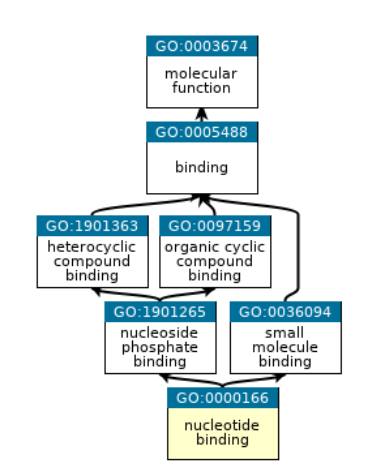
\includegraphics[width=0.6\textwidth]{Figures/go_subgraph.png}
	\caption{Prikaz svih predaka lista označenog funkcijom ‚‚nucleotid binding'' u ontologiji molekulskih funkcija.}
	\label{fig:subgraph}
\end{figure}


\section{Binarni klasifikatori}

Klasifikacija, odnosno, zadatak dodeljivanja objekata jednoj od više predefinisanih kategorija, rasprostranjen je problem koji obuhvata mnoštvo različitih primena. Primeri uključuju otkrivanje spam poruka na osnovu zaglavlja poruke i njenog sadržaja, kategorisanje ćelija kao maligne ili beningne na osnovu rezultata magnetne rezonance, klasifikaciju galaksija na osnovu njihovog oblika, itd. Binarna klasifikacija je slučaj klasifikacije u kojoj postoje tačno dve predefinisane kategorije u koje treba razvrstati date objekte. Obično se za jednu kategoriju kaže da je to pozitivna klasa, a za drugu da je negativna.

Svaki klasifikator upotrebljava algoritam za učenje kako bi odredio model koji najbolje odgovara vezi između skupa atributa i klase ulaznih podataka. Model koji algoritam generiše trebalo bi da odgovara ulaznim podacima kao i da tačno predviđa klasu slogova koje ranije nije video. 


\subsection{Metod potpornih vektora} 

Metod potpornih vektora (engl. \textit{support vector machine}) je tehnika za klasifikaciju zasnovana na ideji vektorskih prostora. Ova metoda generiše klasifikacioni model koji predstavlja funkciju. Osnovni algoritam definisan je za binarnu klasifikaciju.

Osnovna ideja ove metode jeste pronalazak razdvajajuće hiperravni takve da su instance iste klase sa iste strane ravni. Sa tako postavljenim uslovom, razdvajajućih hiperravni može biti više od jedne što je prikazano na slici \ref{fig:svm1}. Iako svaka od ravni razdvaja podatke bez greške, nema garancije da će se podjednako dobro ponašati sa novim podacima koje je potrebno klasifikovati. 


\begin{figure}[H]
	\centering
	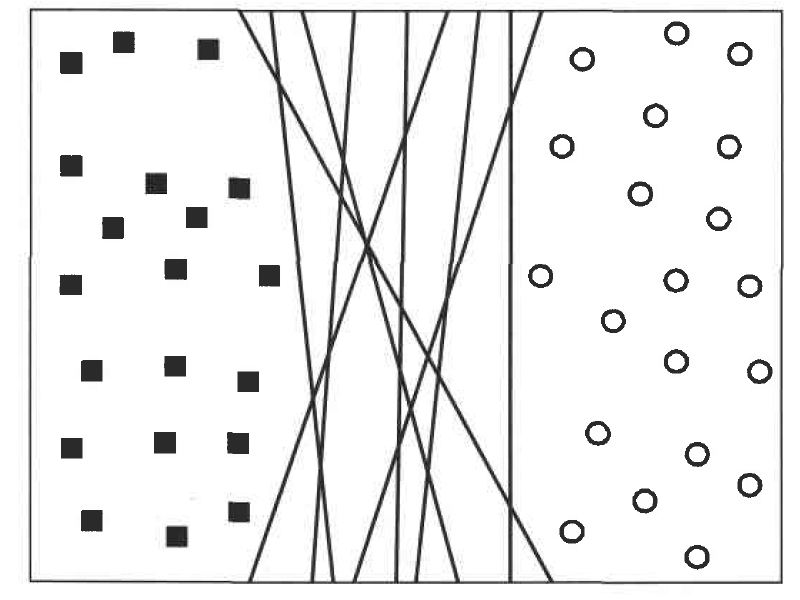
\includegraphics[width=0.6\textwidth]{Figures/svm1.png}
	\caption{Primeri razdvajajućih hiperravni \cite{introDM}.}
	\label{fig:svm1}
\end{figure}


Na slici \ref{fig:svm2} izdvojene su dve hiperravni $B_1$ i $B_2$ i za svaku su dodate dve pomoćne hiperavni $b_{i1}$ i $b_{i2}$. Pomoćne ravni paralelne su glavnoj i pomerene u levu ili desnu stranu do najbliže instance jedne klase. Rastojanje između pomoćnih ravni odnosno rastojanje između najbližih instanci iz obe klase u odnosu na hiperravan naziva se \textit{margina}, a  instance oslonjene na hiperravni su \textit{potporni vektori}. Cilj je pronaći hiperravan koja maksimizuje veličinu margine. Sa slike \ref{fig:svm2} jasno se vidi da je bolja hiperravan $B_1$. Jednačina optimalne hiperravni predstavlja klasifikacioni model. Korak klasifikacije nepoznate instance sastoji se iz izračunavanja njenog rastojanja od hiperravni na osnovu čega se određuje klasa kojoj instanca pripada \cite{introDM, doktJG}.



\begin{figure}[h]
	\centering
	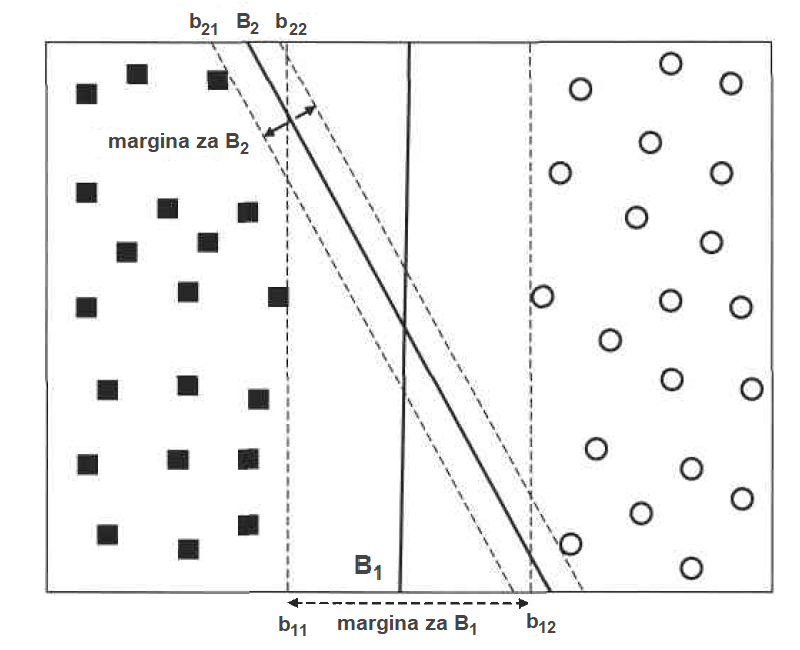
\includegraphics[width=0.6\textwidth]{Figures/svm2.png}
	\caption{Margine razdvajajućih hiperravni \cite{introDM}.}
	\label{fig:svm2}
\end{figure}


Jednačina hiperravni je

$$w \cdot x + w_0 = 0$$

\noindent gde je $w_0$ slobodan član. Na osnovu jednačine rastojanja tačke od hiperravni

$$\dfrac{|w \cdot x + w_0|}{||w||_2}$$

\noindent i činjenice da za svaku od tačaka sa ovih hiperravni važi $w \cdot x + w_0 = 1$, dobija se da je ukupno rastojanje između klasa, u pravcu normalnom u odnosu na optimalnu hiperravan $\dfrac{2}{|w|}$. Tako se optimalna hiperravan dobija pronalaženjem koeficijenata koji maksimizuju ovaj izraz pod uslovima da su sve tačke sa pravih strana te hiperravni odnosno da su podaci linearno razdvojivi. Optimizacioni problem može da se zapiše i kao problem minimizacije i glasi:

$$ \underset{w, w_0}{min} \dfrac{||w||_2}{2}$$
$$ y_i(w \cdot x_i + w_0) \geq 1 \qquad i=1, \ldots, N $$
 
Dodatni uslov će obezbediti da sve tačke budu na većem rastojanju od hiperravni u odnosu na potporne vektore \cite{ml}.

S obzirom da je čest slučaj da podaci nisu linearno razdvojivi potrebno je prihvatiti greške tj. dozvoliti da se neka instanca nađe sa pogrešne strane razdvajajuće hiperravni. U tu svrhu uvode se nove promenljive, $\xi_i$ koje mere koliko je svaka pogrešno klasifikovana instanca udaljena od hiperravni. Taj metod nazivamo metod potpornih vektora sa \textit{mekom marginom}. Optimizacioni problem se menja:

$$ \underset{w, w_0}{min} \dfrac{||w||_2}{2} + C\sum_{i=0}^{N} \xi_i$$
$$ y_i(w \cdot x_i + w_0) \geq 1 - \xi_i \qquad i=1, \ldots, N $$
$$ \xi_i \geq 0  \qquad i=1, \ldots, N $$
 
Metaparametar $C$ kontroliše koliki značaj imaju greške. Ukoliko je vrednost jednaka nuli, onda greške ne igraju nikakvu ulogu, a ako je vrednost velika, onda su greške veoma važne, a pravac hiperravni i širina pojasa nisu bitne \cite{ml}. 


\subsection{Logistička regresija}

Logistička regresija (engl. \textit{logistic regression}) je statistički zasnovan metod za analizu skupa podataka u kom jedna ili više nezavisnih promenljivih određuju ishod. Osnovna pretpostvaka je Bernulijeva rasporedela ciljne promenljive $y$ pri datim vrednostim atributa $x$ odnosno, za date vrednosti atributa $x$, postoji parametar $\mu \in [0, 1]$ tako da važi:

$$ p(y = 1 | x) = \mu $$ 

\noindent odakle je $ p(y=0 | x)$  jednoznačno određeno.
Zadatak je sličan kao prethodnoj metodi, potrebno je pronaći razdvajajuću hiperravan koja deli podatke tako da sa jedne strane budu instance iste klase. Najjaednostavniji je linearan model:

$$f(x) = w \cdot x$$

Međutim, funkcije uzima vrednosti iz intervala $[-\infty, \infty]$ što nije prihvatljivo zbog verovatnoća. Zbog toga se vrednost linearnog modela transformiše monotonom funkcijom u interval $[0, 1]$. U te svrhe, najčešće se koristi sigmoidna funkcija:

$$\sigma(t) = \dfrac{1}{1+exp(-t)}$$

čiji je grafik prikazan na slici \ref{fig:sigmoid}. Nakon transformacije vrednosti linearnog modela sigmoidnom funkcijom, model logističke regresije određen je relacijom:

$$p_w(y = 1 | x) = \sigma(w \cdot x)$$


Iz toga se može odrediti i puna specifikacija problema:

$$p_w(y | x) = \sigma(w \cdot x)^y (1 - \sigma(w \cdot x))^{1-y}$$

Verovatnoća da instanca pripada jednoj klasi je veća što je instanca dalje od hiperravni sa odgovarajuće strane \cite{ml}.

\begin{figure}[h]
	\centering
	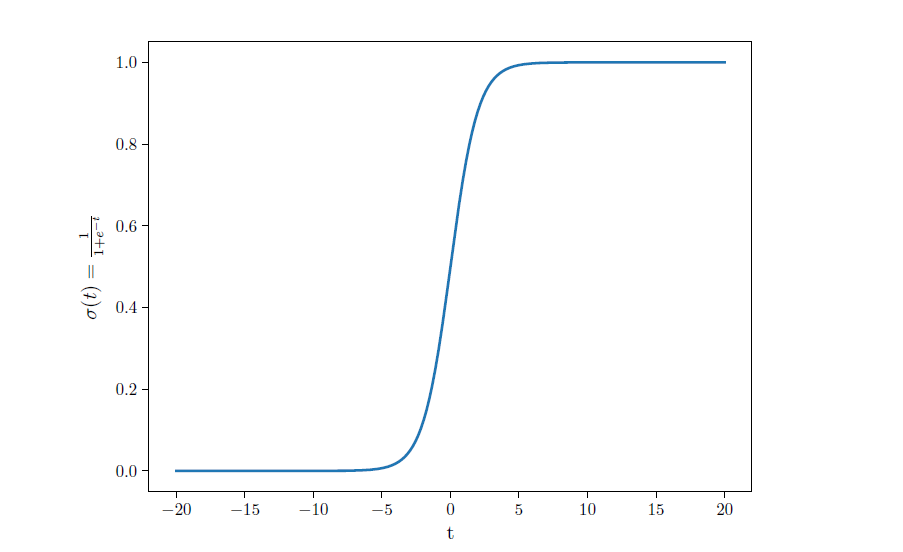
\includegraphics[width=0.8\textwidth]{Figures/sigmoid.png}
	\caption{Grafik sigmoidne funkcije \cite{ml}.}
	\label{fig:sigmoid}
\end{figure}

Ocena parametara ovog modela zasniva se na principu maksimalne verodostojnosti. Uz pretpostavku nezavisnosti instanci, funkcija verodostojnosti zadata je izrazom:

$$\mathcal{L}(w) = \prod_{i=1}^{N}p_w(y_i|x_i)$$

i potrebno je rešiti problem:

$$\underset{w}{max} \mathcal{L}(w)$$

Ukoliko se pređe na negativan logaritam verodostojnosti optimizacioni problem postaje:

$$ \underset{w}{min} -\sum_{i=0}^{N} [y_i\log f_w(x_i) + (1-y_i)\log(1 - f_w(x_i))]$$



\subsection{Slučajne šume} 

Metod slučajne šume (engl. \textit{random forests}) spada u grupu metoda specijalno dizajnirane za stabla odlučivanja. Ona kombinuje predviđanja više različitih stabala, gde je svako stablo generisano na osnovu vrednosti nezavisnog skupa slučajno odabranih vektora.

\subsubsection{Stabla odlučivanja}
 
Problem klasifikacije rešava se postavljanjem pažljivo sastavljenih pitanja o atributima podataka. Pitanja se postavljaju sve dok nije moguće zaključiti klasu date instance. Niz pitanja i odgovora organizovan je u hijerarhijsku strukturu koja se sastoji iz čvorova i direktinih grana. Na slici \ref{fig:tree} je prikazano stablo odlučivanja koje određuje da li je životinja opasna ili ne na osnovu podataka o otrovnosti, veličini i ishrani. 

Svaki list u stablu ima dodeljenu klasu, a unutrašnji čvorovi i koren sadrže uslove koji razdvajaju instance sa različitim karakteristikama. Grane predstavljaju odgovor na pitanje čvora iz kog izlaze. Jednom kada je stablo konstruisano, klasifikacija je jednosmerna. Kreće se od korenog čvora i za konkretnu instancu odgovara se na pitanja koja se nalaze u čvorovima praćenjem odgovarajućih grana sve do listova koje sadrže konačan odgovor. Klasa koja je pridružena listu dodeljuje se instanci \cite{introDM}.


\begin{figure}[h]
	\centering
	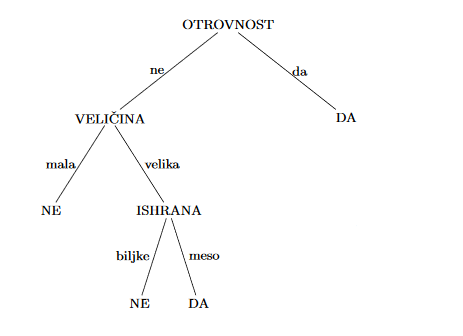
\includegraphics[width=0.7\textwidth]{Figures/tree.png}
	\caption{Primer stabla odlučivanja koje određuje da li je životinja opasna ili ne \cite{vi}.}
	\label{fig:tree}
\end{figure}



\subsubsection{Predviđanje korišćenjem slučajnih šuma} 


Osnovna ideja je kombinovanje više stabala odlučivanja u jedan model. Stabla koja se kombinuju treniraju se nad nezavisnim, slučajno odabranim, podskupovima podataka, a može se koristiti i slučajno odabran podskup atributa. Obučavaju se nad različitim skupovima kako bi njihove greške bile što slabije korelisane \cite{ml}.  
 
Instanca se klasifikuje glasanjem. Svako od konstruisanih stabala klasifikuje instancu u jednu od dve klase, a zatim se svi odgovori broje i odgovor klasifikatora slučajne šume je ona klasa koja ima više glasova tj. ona klasa koju je više stabala predvidelo. Slika \ref{fig:rf} ilustruje proces treniranja i klasifikacije.


\begin{figure}[H]
	\centering
	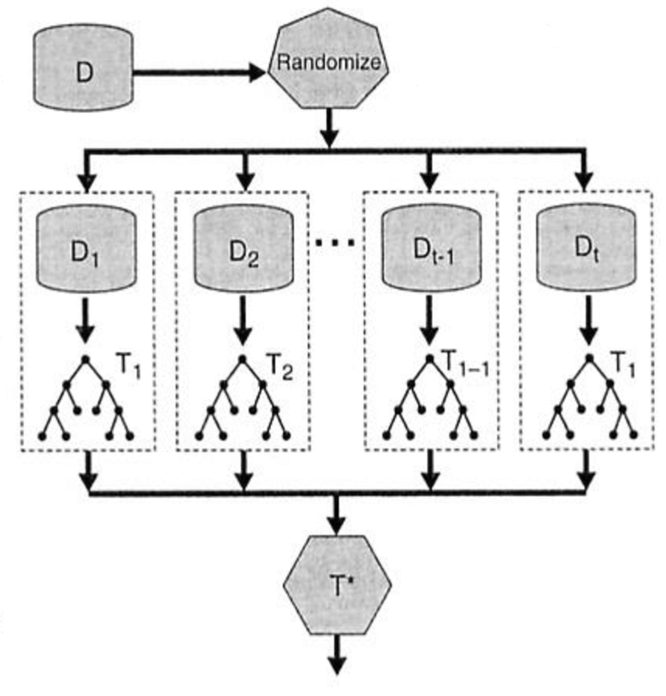
\includegraphics[width=0.6\textwidth]{Figures/random_forests.png}
	\caption{Primer slučajne šume \cite{introDM}. Prvo se iz početnog skupa slučajno odabiraju instance i formira se podskup za svako stablo. Zatim se nad odgovarajućim podskupovima treniraju stabla. Svako stablo klasifikuje nepoznatu instancu i odgovori se kombinuju u jedan, konačan, odgovor modela slučajnih šuma.}
	\label{fig:rf}
\end{figure}
%\chapter{Implementacija predviđanja funkcija proteina}
\label{Chapter5}

Predviđanje funkcije proteina vršeno je metodama binarne klasifikacije i to metodom potpornih vektora, slučajnim šumama i logističkom regresijom. Trenirani su binarni klasifikatori za pojedinačne funkcije ontologije molekulskih funkcija. Ulaz predstavljaju sekvence proteina za koje je određeno da li obavljaju ili ne obavljaju konkretnu funkciju. Odgovor koji svaki od klasifikatora daje je da li zadati protein izvršava odgovarajuću funkciju ili ne.

Kada su svi modeli istrenirani, testirani su nad 100 proteina različitih organizama. Za svaki protein traže se odgovori svih binarnih klasifikatora jedne metode, a njihovi odgovori se spajaju u konačan odgovor - podgraf ontologije koji predstavlja funkciju zadatog proteina.



\section{Podaci}

Podaci o proteinima korišćeni u ovom radu preuzeti su sa adrese \href{https://biofunctionprediction.org/cafa-targets/CAFA3_training_data.tgz}{https://biofunction prediction.org/cafa-targets/CAFA3\_training\_data.tgz}. Oni su podeljeni u dve datoteke:

\begin{enumerate}
	\item \textbf{uniprot\_sprot\_exp.fasta} - proteini i njihove sekvence,
	\item \textbf{uniprot\_sprot\_exp.txt} - proteini i eksperimentalno utvrđene funkcije koje obavljaju.
\end{enumerate}

Dodatne informacije o organizmima iz kojih proteini potiču preuzete su sa \url{https://www.uniprot.org/} i to za organizme:
	\begin{itemize}
		\item čovek (human)
		\item miš (mouse)
		\item pacov (rat)
		\item ešerihija koli (ecoli)
		\item arabidopsis (arath).
	\end{itemize}


Informacije o ontologijama preuzete su sa  \href{http://geneontology.org/docs/download-ontology/}{http://geneontology.org/docs/download-ontology/} u OBO formatu. 

Preuzeti podaci nisu bili u pogodnom obliku za ulaz klasifikatora zbog čega je bilo neophodno njihovo parsiranje.


\paragraph{Ontologija} Datoteka \textit{go.obo} sadrži funkcije iz sve tri ontologije. Njenim parsiranjem izdvojena je ontologija molekulskih funkcija (MFO). Ona se sastoji iz približno 12000 čvorova, međutim, neki čvorovi su zastareli (\textit{engl. obsolete}) zbog čega su izbačeni iz grafa. Pored toga, postoje čvorovi koji predstavljaju alternativni identifikator nekog drugog čvora te su takvi čvorovi ujedinjeni u jedan. Time je broj čvorova smanjen na 11078 molekulskih funkcija. Broj je dodatno umanjen zbog prirode podataka. Pre svega, približno 5500 funkcija se uopšte ne pojavljuje u trening skupu što znači da za njih nema pozitivnih instanci odnosno proteina koji ih izvršavaju pa su one izbačene. Zatim, oko 5000 funkcija se pojavljuje manje od 100 puta u trening skupu. Pokušaji treninga klasifikatora za takve funkcije su bili neuspešni te su i one izbačene iz skupa. Nakon svih redukcija ostalo je 399 funkcija sa 100 ili više pojavljivanja u trening skupu za koje su trenirani modeli.


\paragraph{Proteini i funkcije} Parsiranjem \textit{uniprot\_sprot\_exp.txt} izdvojeno je više informacija - proteini sa funkcijama koje obavljaju kao i funkcije sa proteinima za koje je utvrđeno da ih obavljaju. Prvi skup podataka je obogaćen podacima iz ontologije s obzirom da su zadati samo krajnji čvorovi, a ne i svi preci, kako bi se dobio ceo podgraf ontologije koji predstavlja funkciju proteina. Drugi skup poslužio je za prebrojavanje pojavljivanja funkcije u trening skupu kao i za kasnije formiranje skupa pozitivnih i negativnih instanci.


\paragraph{Sekvence proteina} U datoteci \textit{uniprot\_sprot\_exp.fasta} 
nalazi se 66817 proteina. Među njima se nalaze i proteini koji ne obavljaju neku od funkcija iz MFO. Pored toga, postoje proteini čije sekvence nisu validne u smislu aminokiselina koje sadrže. Pod validnim sekvencama podrazumevaju se samo one koje se sastoje isključivo iz 20 standardnih aminokiselina. Nakon eliminacije ovakvih proteina preostaje 34785 onih koji obavljaju bar jednu molekulsku funkciju. Nakon redukcije broja funkcija na 399 smanjio se i skup proteina. Naime, izbačeni su svi proteini za koje je utvrđeno da vrše neku od eliminisanih funkcija. Nakon svih redukcija, veličina trening skupa je 20960. 



\subsection{Predstavljanje proteina}
\label{subsec:proteins}

Mnoge metode mašinskog učenja koriste vektore kao ulaz zbog čega je pogodno da se niska aminokiselina prepiše u niz. Jedan pogodan način za to jeste prebrojavanjem pojavljivanja svakog mogućeg trigrama nad azbukom 20 standardnih aminokiselina. Dimenzija jednog niza je samim tim $20^3$, a jedan element sadrži broj pojavljivanja odgovarajućeg trigrama u niski aminokiselina. Ono što je neophodno jeste da za svaki trigram postoji jedinstveno određen redni broj u nizu. U te svrhe, prvo je potrebno odrediti brojeve pojedinačnih aminokiselina, a šema korišćena u ovoj implementaciji prikazana je u tabeli \ref{tab: aminosNumbers}.


\begin{table}[H]
	\centering
	\begin{tabular}{|c|c|c|c|c|c|c|c|c|c|c|c|c|c|c|c|c|c|c|c|}
		\hline
		A & C & D & E & F & G & H & I & K & L & M & N & P & Q & R & S & T & V & W & Y \\
		\hline
		0 & 1 & 2 & 3 & 4 & 5 & 6 & 7 & 8 & 9 & 10 & 11 & 12 & 13 & 14 & 15 & 16 & 17 & 18 & 19 \\
		\hline             
	\end{tabular}
	\caption{Preslikavanje aminokiselina u broj}
	\label{tab: aminosNumbers}
\end{table}

Sada, za svaki trigram može da se odredi njegov jedinstveni broj koji predstavlja poziciju u nizu i to formulom:

$$kmer\_index = aa_1*20^2 + aa_2 * 20 + aa_3$$

Sa ovakvim preslikavanjem trigrama u brojeve, jednostavnim prolaskom kroz nisku sa korakom od 3 karaktera dobija se odgovarajući niz.


\section{Treniranje modela}
\label{sec:train}


Program je pisan u programskom jeziku Python i korišćene su implementacije metoda binarne klasifikacije iz Python-ove biblioteke \textit{sklearn}. Trenirano je 399 modela za svaki metod pojedinačno. Početni skup proteina podeljen je na trening i test skup u razmeri 3:1. Tokom treniranja izvršen je i odabir modela na validacionom skupu koji je izdvojen iz trening skupa u istoj razmeri. Odabir najboljeg modela izvršen je na osnovu f1-mere.

Nakon što je obučavanje jednog modela završeno, on je sačuvan u posebnoj datoteci sa nazivom koji odgovara identifikatoru funkcije za koju je model treniran i to korišćenjem još jedne Python-ove biblioteke - \textit{pickle}. Ova biblioteka omogućava čuvanje i kasnije čitanje modela mašinskog učenja u pogodnom obliku, tako da nema potrebe za obučavanjem ispočetka već su modeli odmah spremni za predviđanje.


\paragraph{Metod potpornih vektora}

Prilikom odabira modela birana je vrednost za parametar C i to iz skupa $\{0.01, 0.1, 1, 10\}$. Pored toga, odabiran je bolji od dva kernela, linearan i gausov. Zbog dugačkog treniranja jednog modela i velikog broja modela koje je trebalo obučiti, svim nizovima redukovana je dimenzionalnost na 1000. U te svrhe korišćena je Python-ova implementacija algoritma analize glavnih komponenti iz biblioteke \textit{sklearn}.  



\paragraph{Logistička regresija}

Prilikom odabira modela birana je vrednost za parametar C i to iz skupa $\{0.0001, 0.001, 0.01, 0.1, 1\}$. Neki modeli nisu uspevali da nauče ništa iz podataka i njihova f1-mera bila je jednaka 0. Za takve modele izvršen je dodatan trening na proširenom skupu podataka. Proširenje skupa se odnosi na generisanje sintetičkih instanci kako bi se ublažila nebalansiranost pozitivnih i negativnih instanci. Za proširivanje skupa korišćena je Python-ova biblioteka \textit{imblearn}, a skup je obogaćen tako da odnos pozitivnih i negativnih instanci bude 1:2.


\paragraph{Slučajne šume}

Kod modela slučajnih šuma trenirani su modeli sa različitim brojem stabala iz skupa $\{100, 400, 700, 1000\}$. Slično kao kod logističke regresije, za modele čija je f1-mera bila 0 izvršen je dodatan trening sa dodatnim pozitivnim instancama.



\section{Objedinjavanje modela}

Nakon što su svi modeli za odabrani metod obučeni prelazi se na testiranje. Izdvojen je skup od 100 proteina nad kojim je testiran prediktor. Prediktor je formiran na osnovu 399 prethodno obučenih modela koji se na samom početku učitavaju u memoriju. Prilikom predviđanja funkcije jednog proteina, protein se prosleđuje kao ulaz svakom od binarnih klasifikatora koji daju vrednosti 0 ili 1. Ujedinjavanjem svih odgovora dobija se konačan odgovor. Sve funkcije za koje je odgovarajući klasifikator dao 1 kao odgovor predstavljaju čvor podgrafa.



\section{Evaluacija modela}

Kao mera kvaliteta pojedinačnih modela korišćena je $f_1$ mera. U okviru biblioteke \textit{sklearn} implementirana je funkcija koja određuje ovu vrednost na osnovu pravih i predviđenih klasa instanci iz test skupa. 

Ista mera korišćena je za evaluaciju konačnog prediktora koji ujedinjuje sve odgovore. S obzirom da prediktor daje strukturu kao odgovor (usmereni aciklički graf) treba preciznije definisati kako se ova mera određuje. Pretpostavimo da je datoj test instanci pridružen izlazni vektor $y = [0, 1, 1, 0, 1, 1]$, a da je prediktor dao odgovor $y' = [0, 0, 1, 1, 0, 1]$ za istu test instancu. Poređenjem dva vektora može se lako utvrditi koje su klase ispravno određene, a koje pogrešno odnosno mogu se odrediti veličine $tp$, $tn$, $fp$ i $fn$ opisane u sekciji \ref{sec:evaluation}:

$$y' = [\underset{\in tn}{0}, \underset{\in fn}{0}, \underset{\in tp}{1}, \underset{\in fp}{1}, \underset{\in fn}{0}, \underset{\in tp}{}]$$

\noindent Na osnovu ovih veličina dalje se mogu odrediti preciznost i odziv, a onda i  $f_1$ mera.





%\chapter{Rezultati} % Main chapter title
\label{Chapter6}

Za svaki od tri prethodno opisana metoda binarne klasifikacije trenirano je po 398 modela na celom trening skupu koji su kasnije ujedinjeni u 3 prediktora za predviđanje funkcije proteina. Implementiran je još jedan jednostovaniji klasifikator koji je poslužio kao osnovna metoda za poređenje rezultata. U pitanju je naivni klasifikator koji svakom čvoru dodeljuje vrednost koja odgovara njegovoj frekvenciji pojavljivanja u trening skupu i tako formirani graf pridružuje svakom test primeru \cite{doktJK}. 

Naivni klasifikator je testiran na istom test skupu kao i 3 prediktora pri čemu su određene prosečne vrednosti za 5 mera kvaliteta modela i to $f_1$-mera, tačnost, preciznost, odziv i površina ispod ROC krive. Prilikom svakog testiranja računata je prosečna vrednost svake mere kvaliteta i to na nivou pojedinačnih organizama, kao i na nivou celog skupa. 

Sa slike \ref{fig:f1scores} se može videti da je svaki od tri prediktora bolji od naivnog klasifikatora prema $f1$-meri. Pored toga, sva 3 prediktora na celom skupu imaju približnu $f1$-meru. Nešto slabiji rezultat metode potpornih vektora mogu se objasniti primenom analize glavnih komponenti na trening skup čime je izgubljen deo informacija. 


Poređenje tačnosti, prikazano na slici \ref{fig:accscores}, pokazuje da svi modeli imaju sličnu tačnost, što može biti posledica nebalansiranog skupa podataka jer je visoka tačnost postignuta zbog velikog broja ispravno klasifikovanih negativnih instanci, a pošto je skup nebalansiran u korist negativne klase, većina instanci je dobro klasifikovana. Prema preciznosti (slika \ref{fig:prescores}) se ističu modeli metode slučajne šume, dok su prema odzivu (slika \ref{fig:recscores}) bliski klasifikatori metode potpornih vektora i logističke regresije. Sa svih grafika na slici \ref{fig:eval} vidi se da su rezultati konzistentni za sve organizme. Na primer, predviđanje funkcija proteina čoveka ne daje bolje rezultate nego predviđanje funkcija proteina za ostale organizme.


U tabelama \ref{tab: rfF1}, \ref{tab: lrF1} i \ref{tab: svmF1} za 20 najboljih\footnote{Najboljih prema vrednosti za $f1$-meru.} pojedinačnih klasifikatora za svaku upotrebljenu metodu binarne klasifikacije prikazane su vrednosti za $f_1$-meru, tačnost, preciznost, odziv, površinu ispod krive, kao i nivo na kom se čvor nalazi u grafu, broj i procenat pojavljivanja funkcije u trening skupu. Pored toga, prikazan je i broj pojavljivanja u trening skupu za svaku funkciju, kao i udeo broja pojavljivanja funkcije u celom trening skupu. Vrednosti za sve klasifikatore prikazane su na adresi \url{http://poincare.matf.bg.ac.rs/~anja_bukurov/master/}.


\begin{figure}[H]
	\begin{subfigure}{0.9\textwidth}
		\centering
		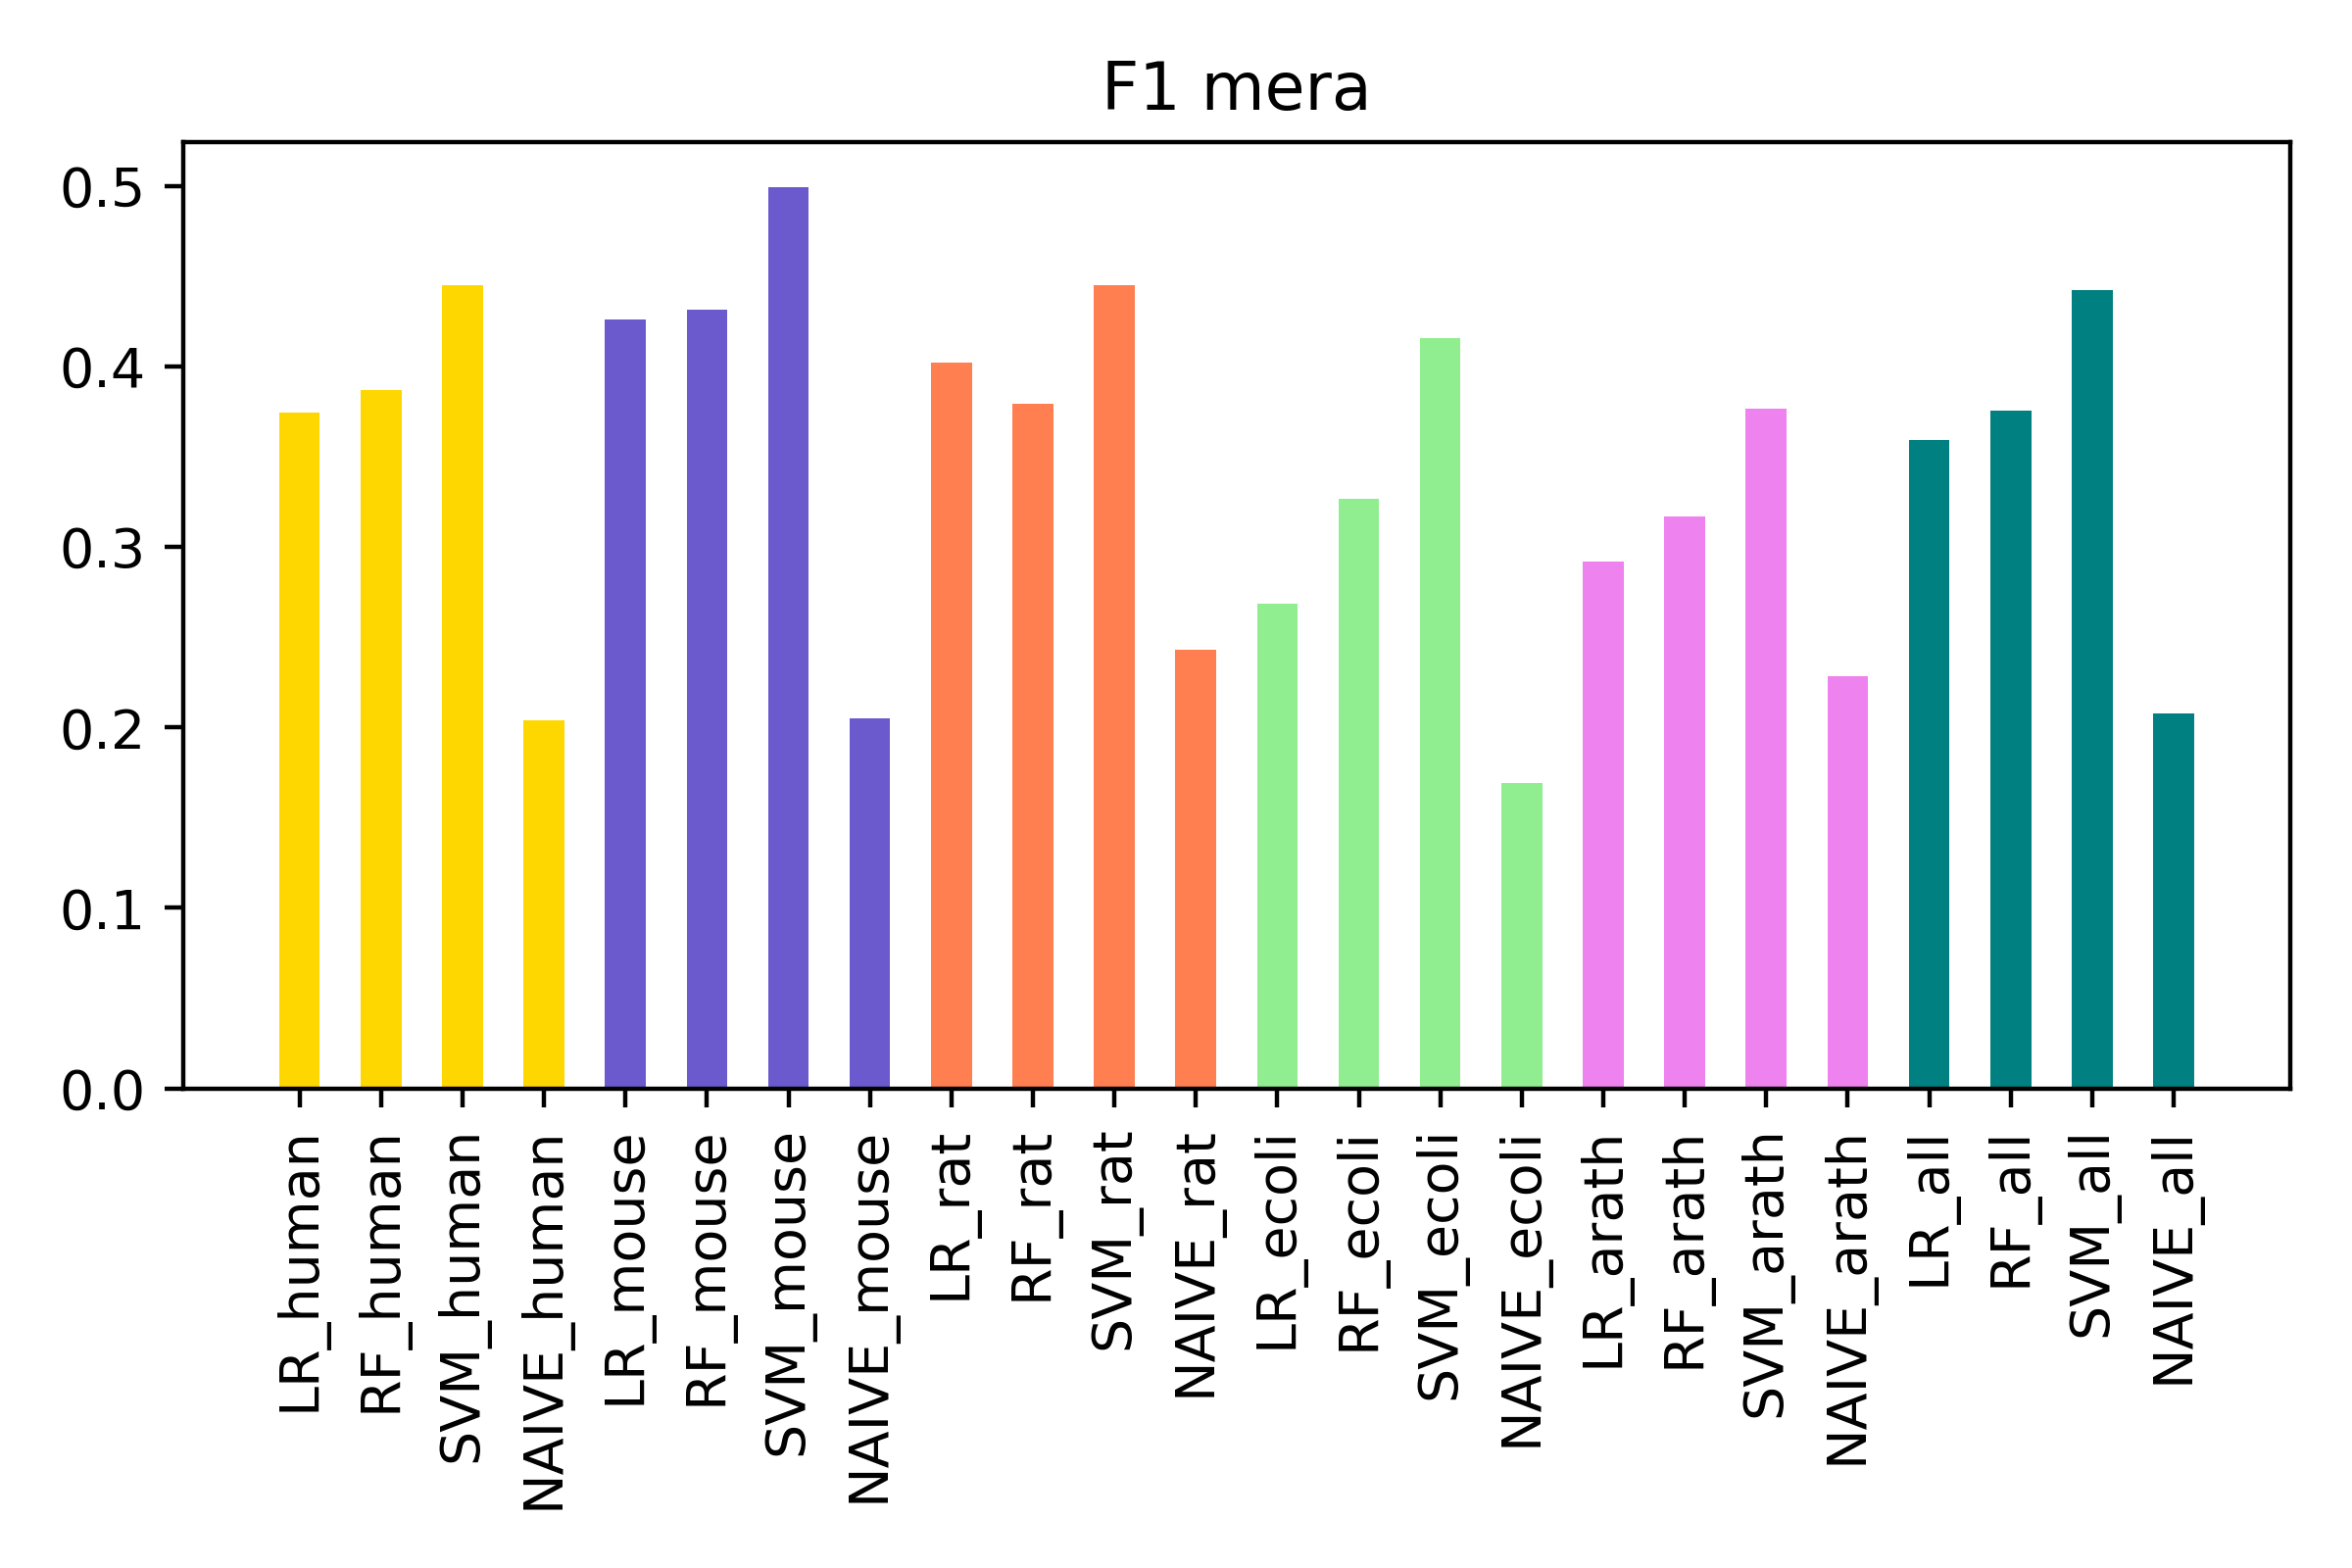
\includegraphics[width=\textwidth]{Figures/f1_poredjenje.png}
		\caption{Poređenje prediktora i naivnog klasifikatora prema f1-meri.}
		\label{fig:f1scores}
	\end{subfigure}

	\begin{subfigure}{0.5\textwidth}
		\centering
		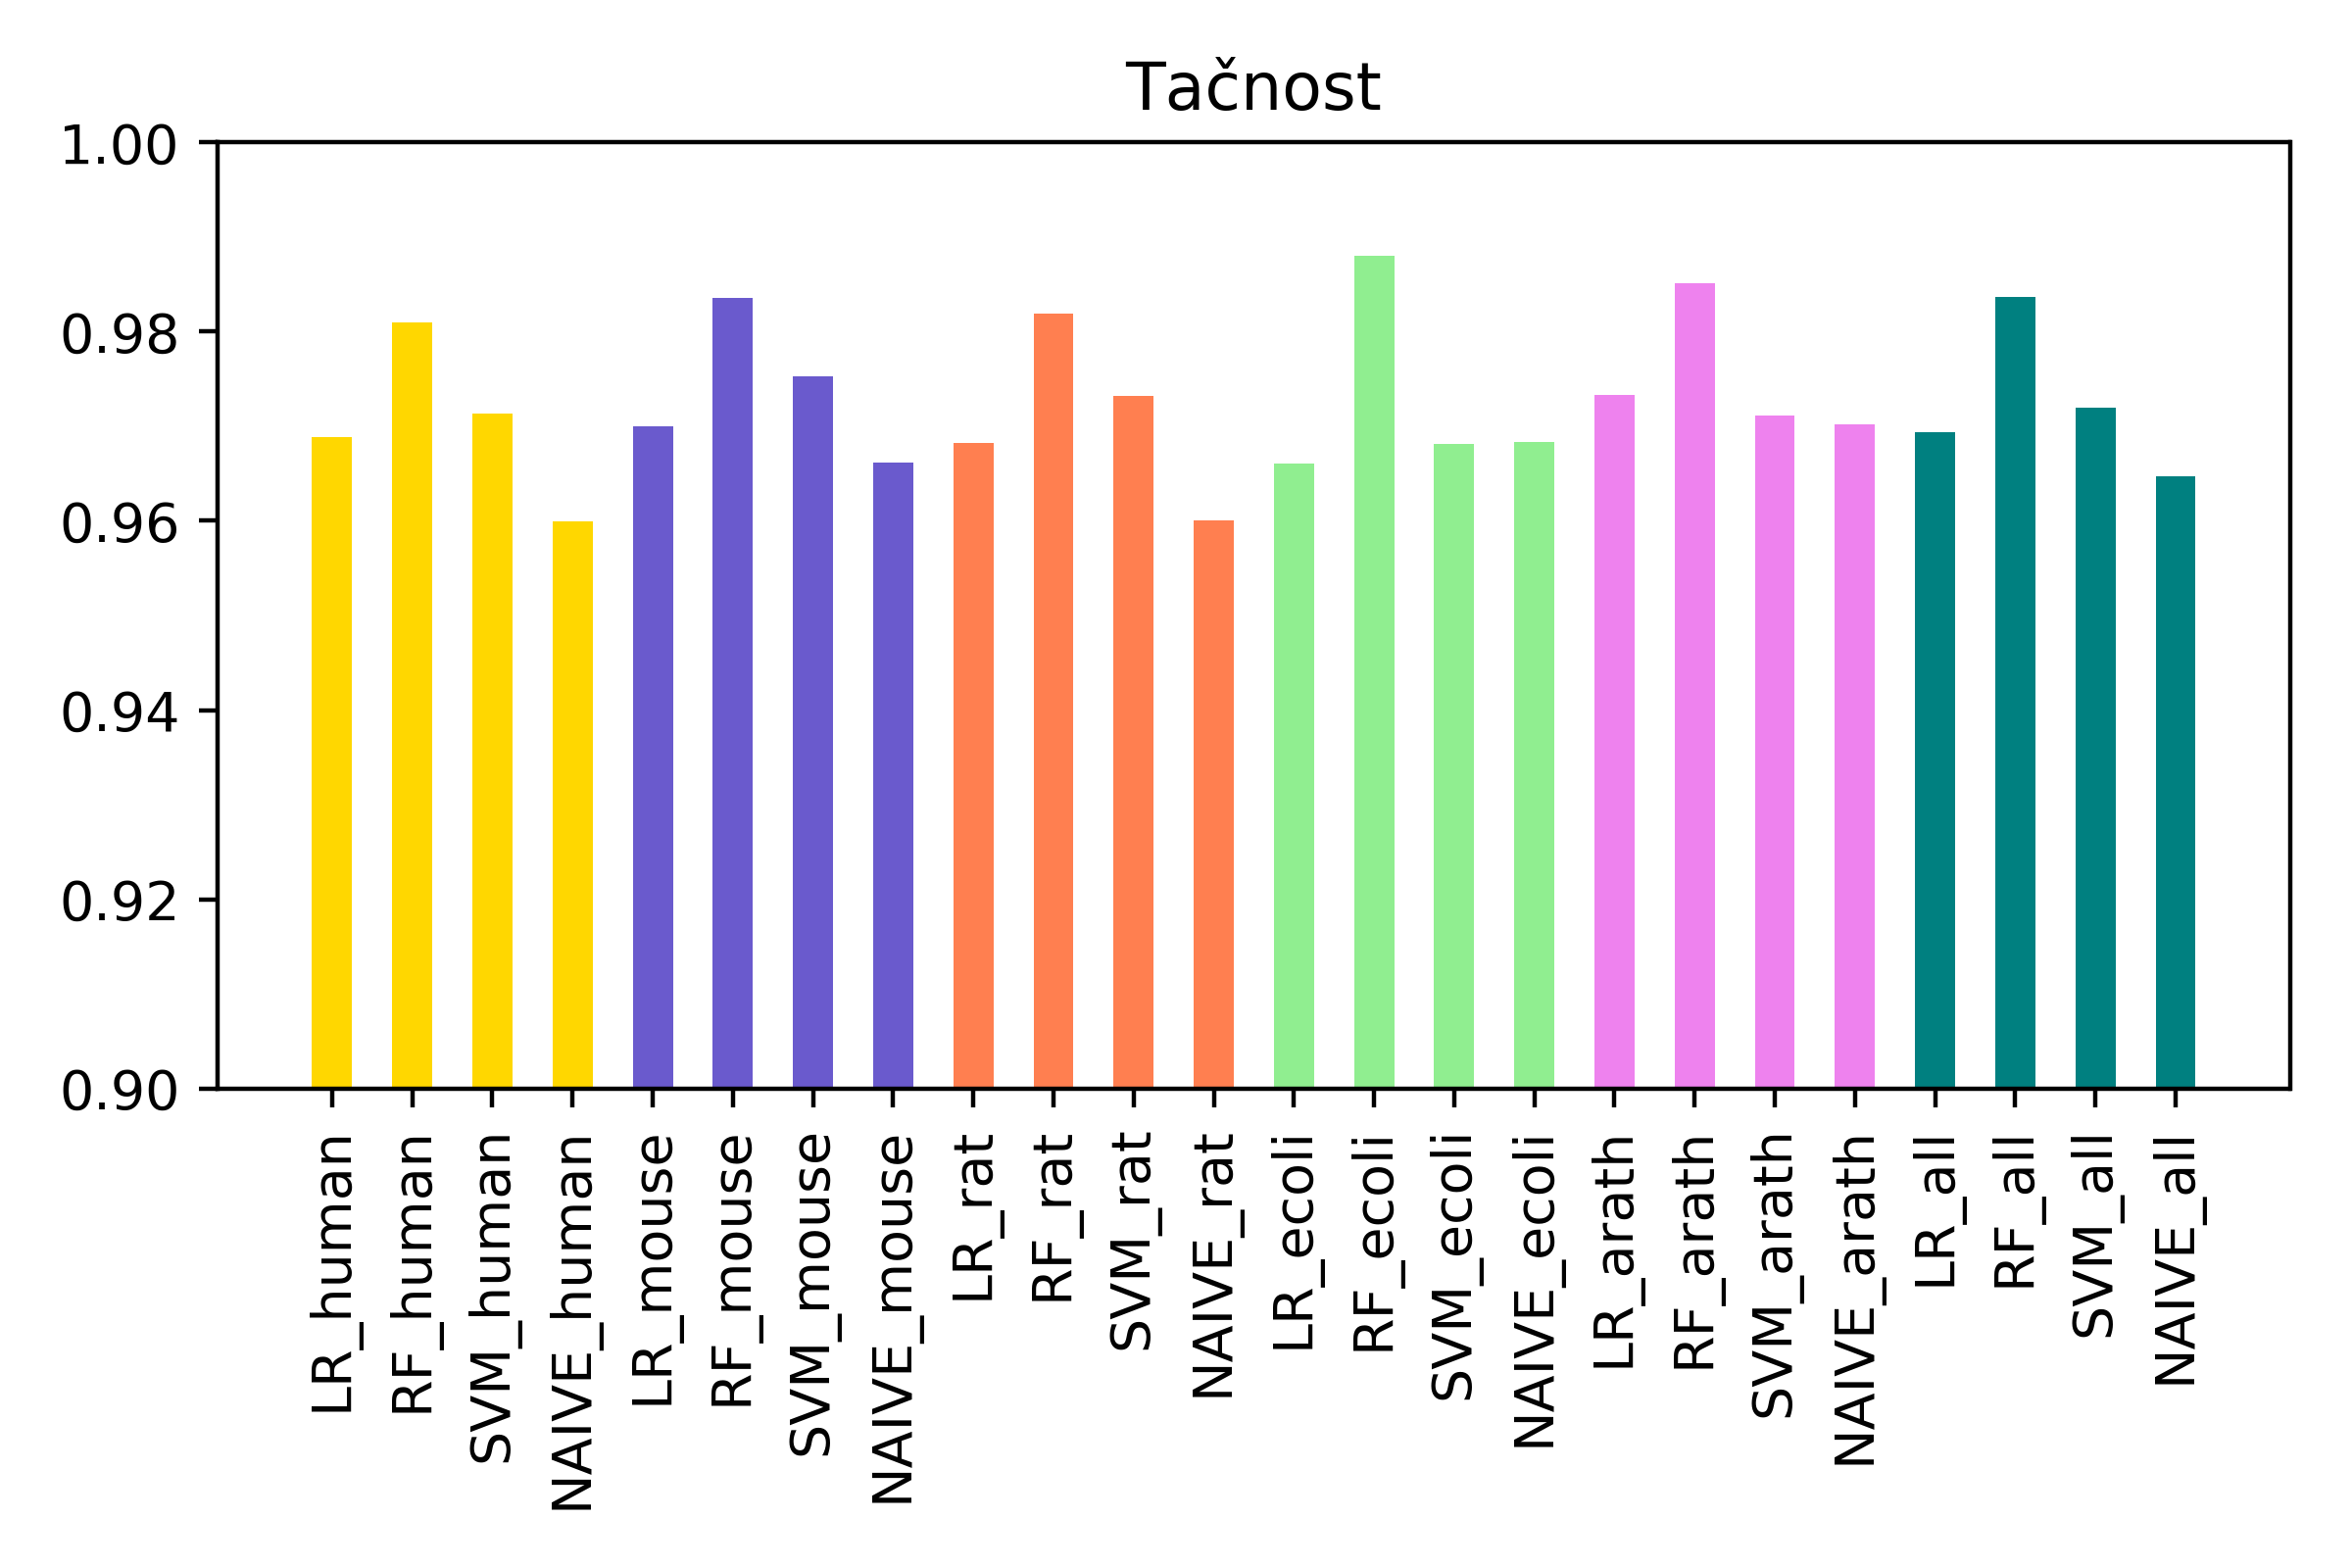
\includegraphics[width=\textwidth]{Figures/acc_poredjenje.png}
		\caption{Poređenje prema tačnosti. }
		\label{fig:accscores}
	\end{subfigure}
	\begin{subfigure}{0.5\textwidth}
		\centering
		% include second image
		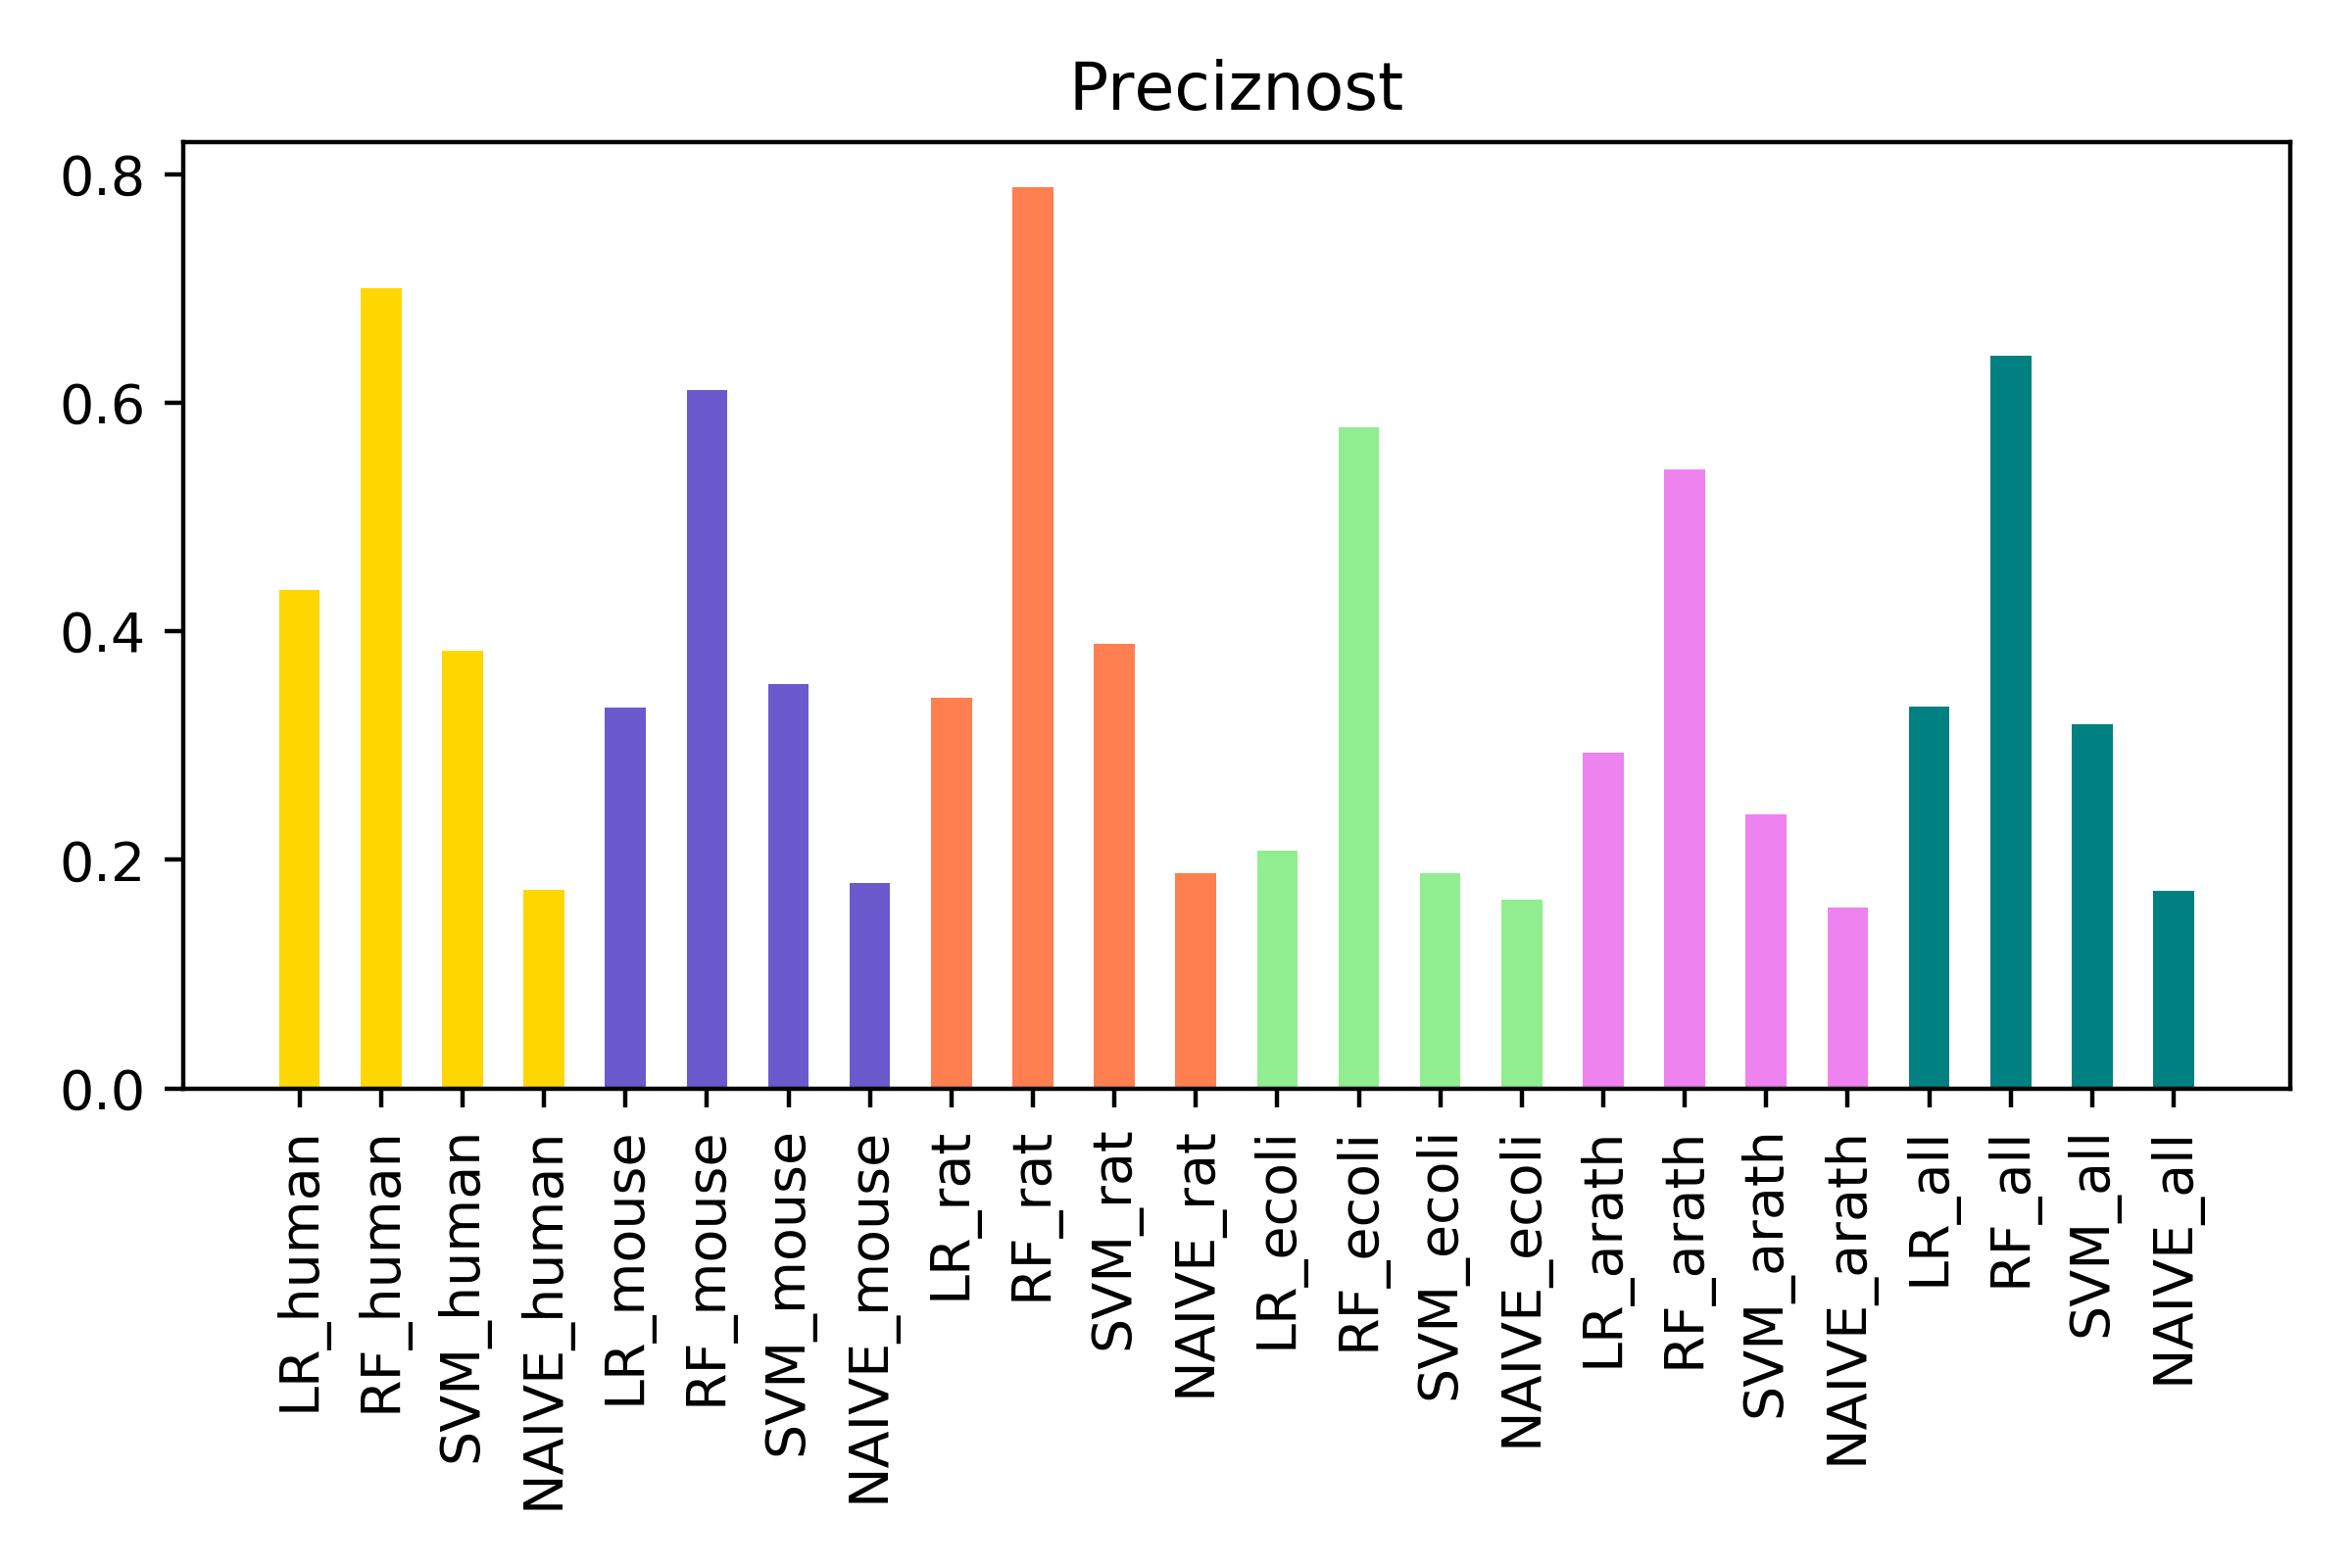
\includegraphics[width=\textwidth]{Figures/pre_poredjenje.png}
		\caption{Poređenje prema preciznosti. }
		\label{fig:prescores}
	\end{subfigure}

~
	\newline
	\newline
~

	\begin{subfigure}{0.5\textwidth}
		\centering
		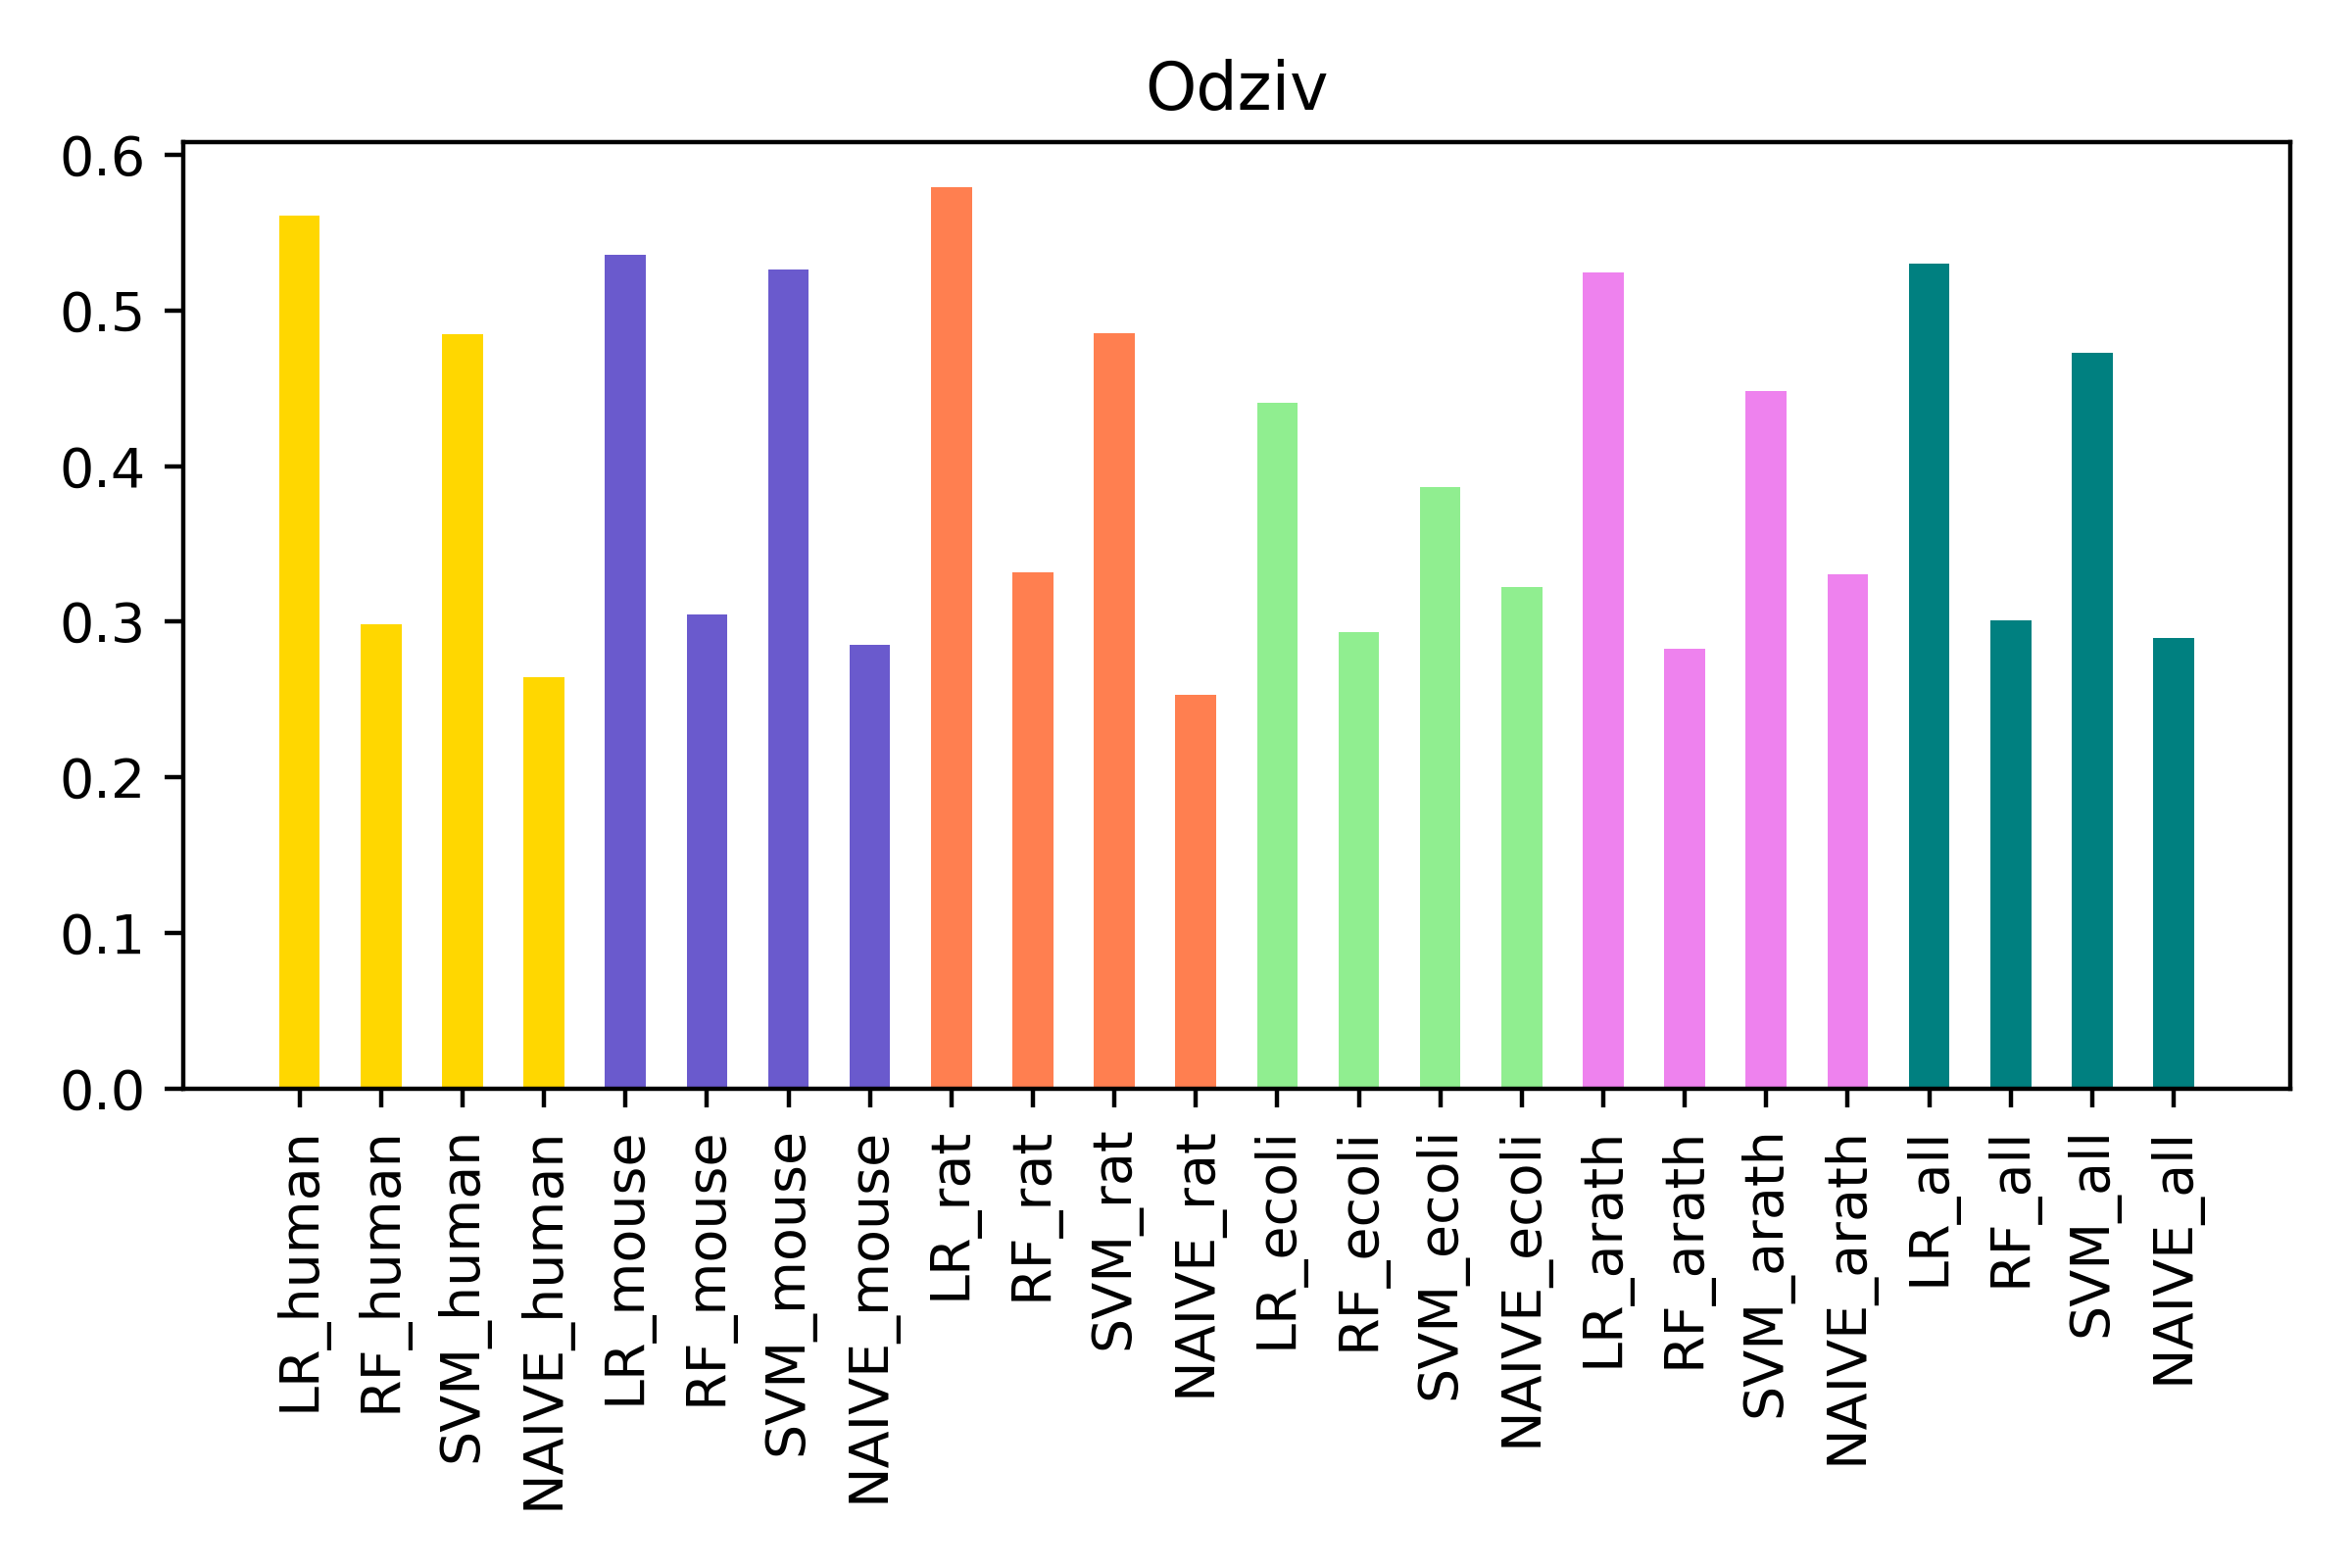
\includegraphics[width=\textwidth]{Figures/rec_poredjenje.png}
		\caption{Poređenje prema odzivu.}
		\label{fig:recscores}
	\end{subfigure}
	\begin{subfigure}{0.5\textwidth}
		\centering
		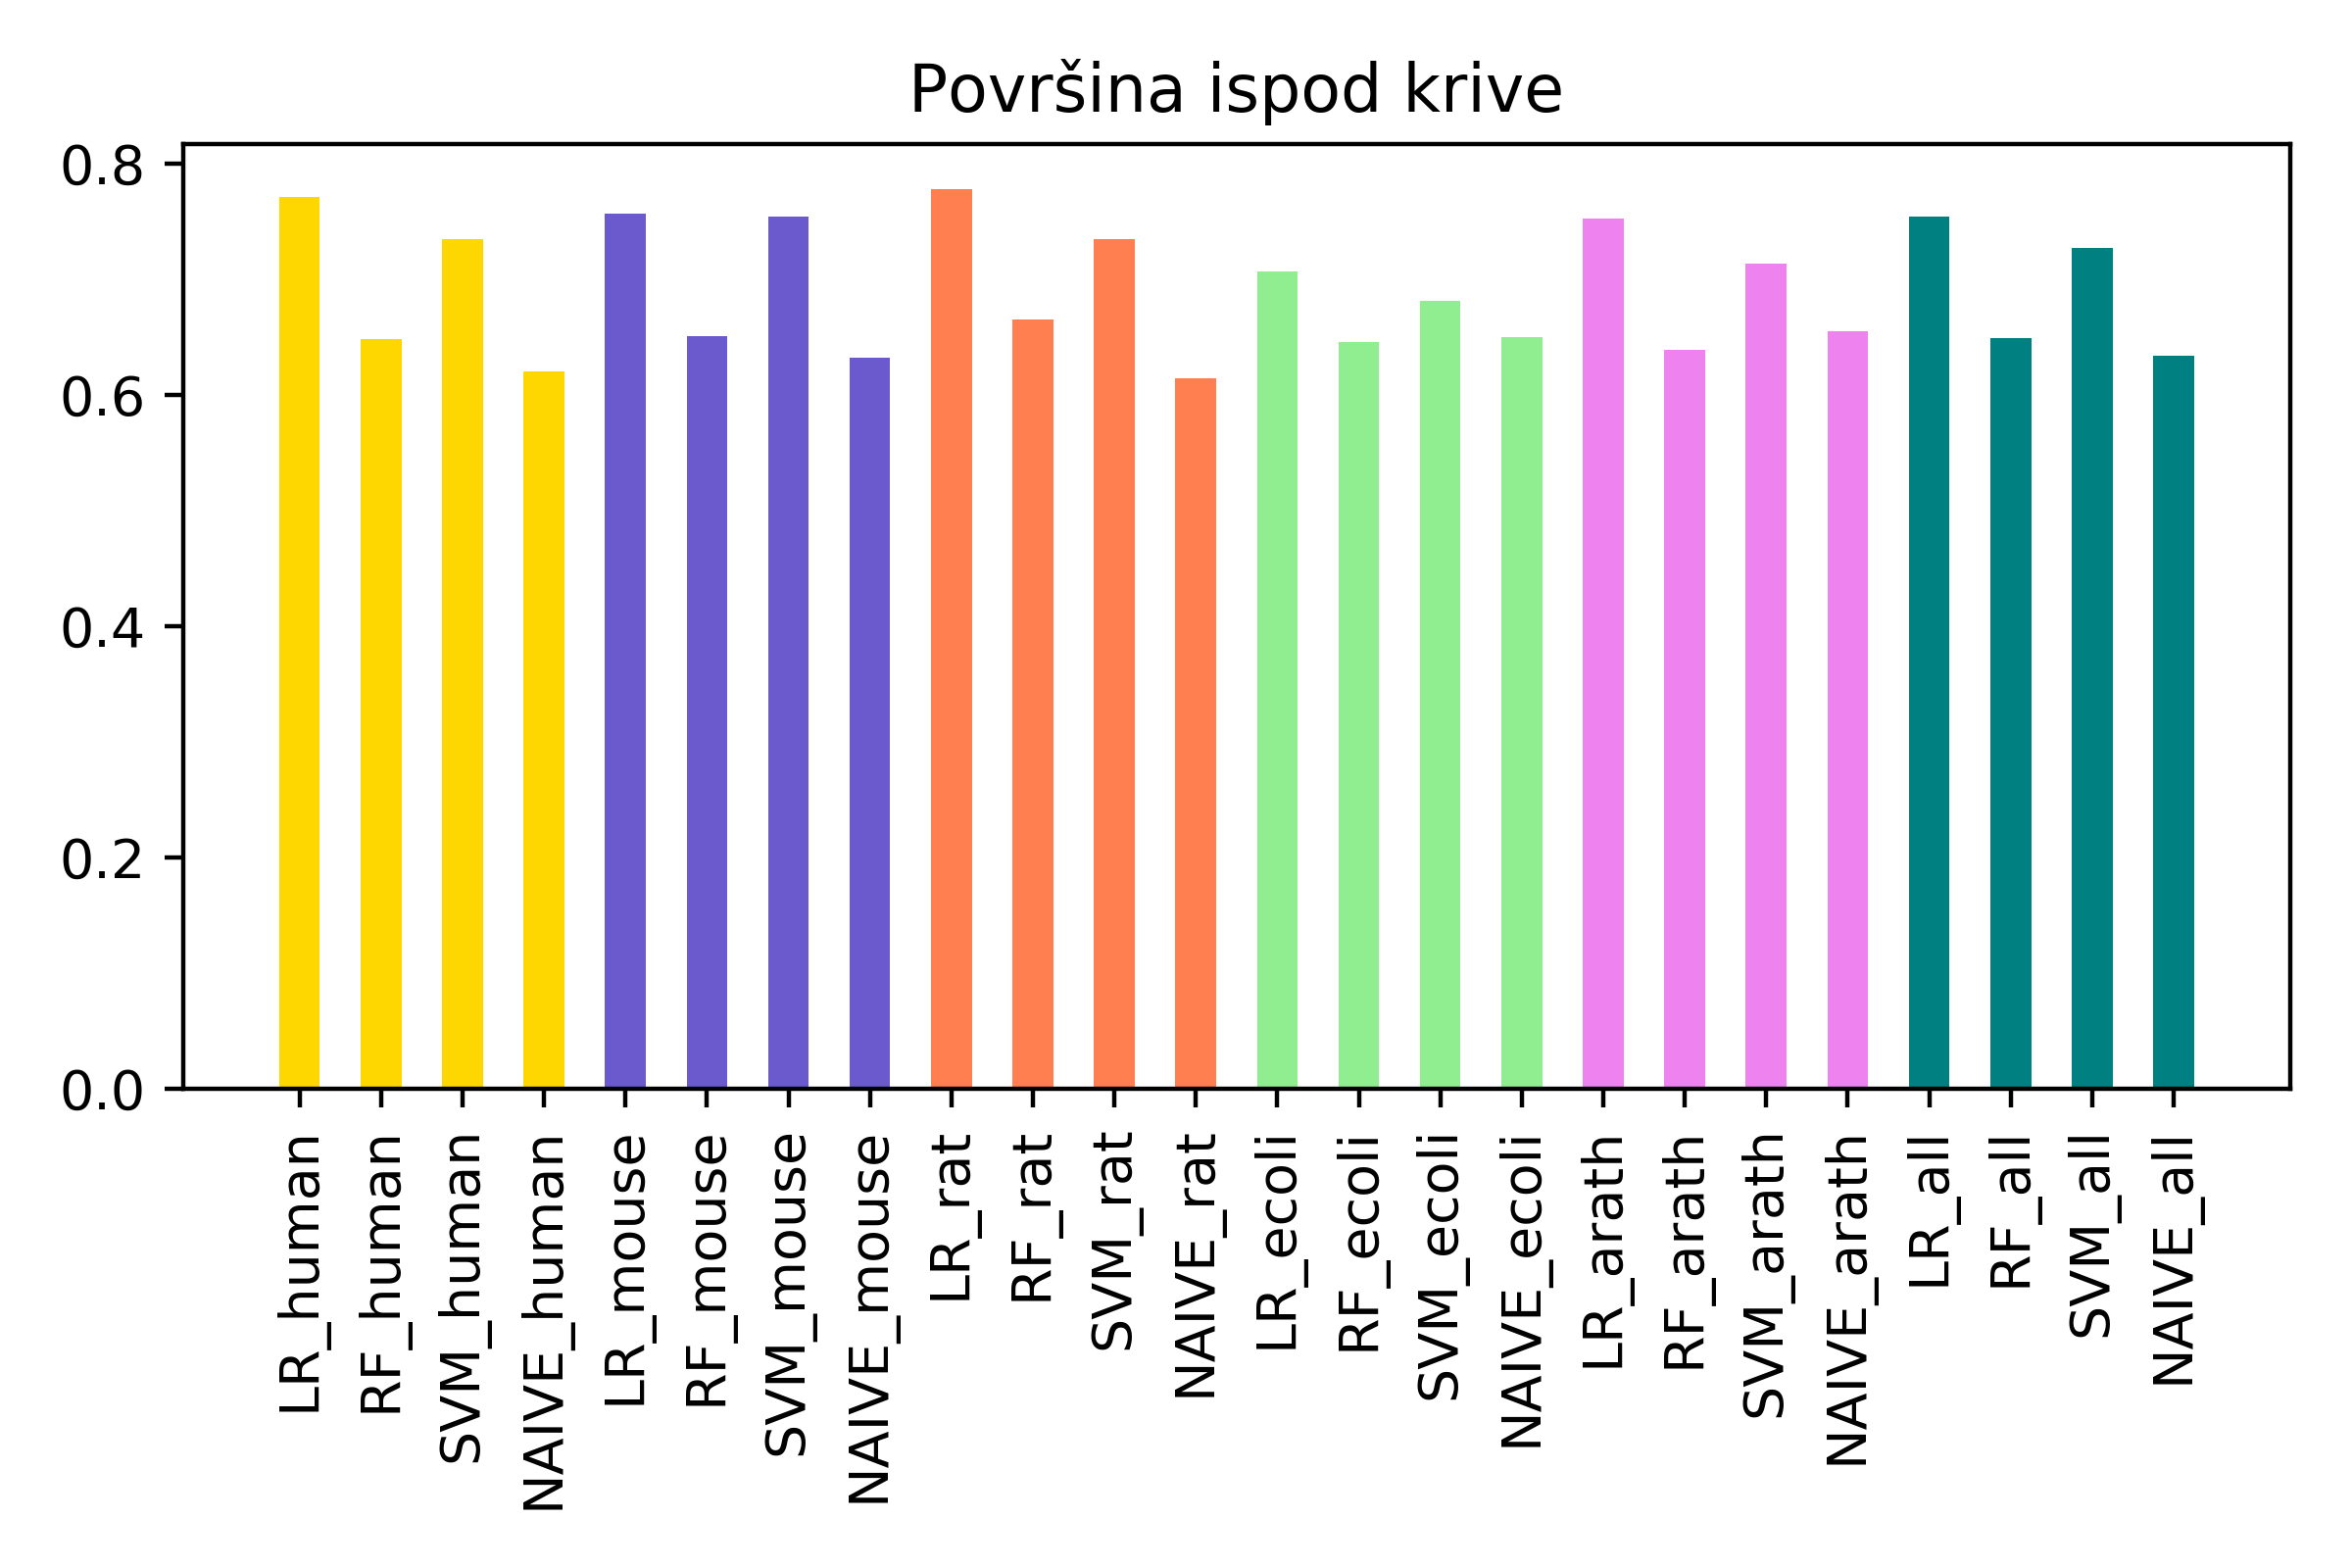
\includegraphics[width=\textwidth]{Figures/auc_poredjenje.png}
		\caption{Poređenje prema površini ispod ROC krive.}
		\label{fig:aucscores}
	\end{subfigure}
	\caption{Poređenje mera kvaliteta prediktora i naivnog klasifikatora. Rezultati jednog organizma prikazani su istom bojom.}
	\label{fig:eval}
\end{figure}

\begin{table}[h]
	\centering
	\begin{tabular}{|c|c|c|c|c|c|c|c|c|}
		\hline
		Funkcija & F1 & Acc & Pre & Rec & AUC & Nivo & Br. p. & Pr. p. \\
		\hline
		GO:0005488 & 0.84 & 0.731 & 0.74 & 0.97 & 0.54 & 1 & 15092 & 72.3\% \\
		\hline
		GO:0017171 & 0.57 & 0.991 & 0.91 & 0.42 & 0.71 & 4 & 354 & 1.7\% \\
		\hline
		GO:0016825 & 0.56 & 0.991 & 0.91 & 0.4 & 0.7 & 3 & 354 & 1.7\% \\
		\hline
		GO:0008236 & 0.54 & 0.991 & 0.93 & 0.38 & 0.69 & 5 & 349 & 1.7\% \\
		\hline
		GO:0004672 & 0.53 & 0.961 & 0.92 & 0.37 & 0.69 & 3 & 1257 & 6.0\% \\
		\hline
		GO:0003824 & 0.52 & 0.738 & 0.84 & 0.37 & 0.67 & 1 & 7843 & 37.6\% \\
		\hline
		GO:0016773 & 0.51 & 0.955 & 0.94 & 0.35 & 0.67 & 4 & 1377 & 6.6\% \\
		\hline
		GO:0016301 & 0.47 & 0.95 & 0.96 & 0.31 & 0.65 & 4 & 1452 & 7.0\% \\
		\hline
		GO:0016772 & 0.46 & 0.943 & 0.96 & 0.31 & 0.65 & 3 & 1609 & 7.7\% \\
		\hline
		GO:0004674 & 0.44 & 0.974 & 0.8 & 0.3 & 0.65 & 4 & 776 & 3.7\% \\
		\hline
		GO:0140096 & 0.42 & 0.88 & 0.89 & 0.27 & 0.63 & 2 & 3337 & 16.0\% \\
		\hline
		GO:0016740 & 0.36 & 0.881 & 0.92 & 0.23 & 0.61 & 2 & 3069 & 14.7\% \\
		\hline
		GO:0030594 & 0.32 & 0.998 & 0.75 & 0.2 & 0.6 & 3 & 86 & 0.4\% \\
		\hline
		GO:1901363 & 0.3 & 0.735 & 0.73 & 0.19 & 0.58 & 2 & 6236 & 29.9\% \\
		\hline
		GO:0016787 & 0.23 & 0.864 & 0.77 & 0.13 & 0.56 & 2 & 3202 & 15.3\% \\
		\hline
		GO:0019199 & 0.17 & 0.996 & 0.67 & 0.1 & 0.55 & 4 & 78 & 0.4\% \\
		\hline
		GO:0060089 & 0.16 & 0.957 & 0.72 & 0.09 & 0.54 & 1 & 976 & 4.7\% \\
		\hline
		GO:0038023 & 0.11 & 0.959 & 0.72 & 0.06 & 0.53 & 2 & 909 & 4.4\% \\
		\hline
		GO:0004888 & 0.11 & 0.971 & 0.75 & 0.06 & 0.53 & 3 & 626 & 3.0\% \\
		\hline
		GO:0004930 & 0.09 & 0.984 & 0.8 & 0.05 & 0.52 & 4 & 312 & 1.5\% \\
		\hline
	\end{tabular}
	\caption{Prikaz mera kvaliteta za pojedina\v cne klasifikatore metode slučajne šume za 20 \v cvorova sa najboljom $f1$-merom}
	\label{tab: rfF1}
\end{table}


Klasifikatori se odlikuju visokom preciznošću, ali niskim odzivom što znači da većinu instanci klasifikuju kao negativne, ali one koje su klasifikovane kao pozitivne su uglavnom ispravno klasifikovane. Tačnost ovih modela je visoka (oko 0.9 i više) za funckije sa manjim brojem pozitivnih instanci (ispod 10\%), dok je za funkcije sa većim brojem instanci nešto tačnost nešto manja (ispod 0.8). Slika \ref{fig:rf_ontology} ilustruje podgraf ontologije koji sadrži funkcije ove tabele.


\begin{figure}[H]
	\centering
	\includegraphics[width=\textwidth]{Figures/RFo.png}
	\caption{Prikaz podgrafa ontologije koji sadrži funkcije iz tabele \ref{tab: rfF1}}
	\label{fig:rf_ontology}
\end{figure}

\begin{table}[h]
	\centering
	\begin{tabular}{|c|c|c|c|c|c|c|c|c|}
		\hline
		Funkcija & F1 & Acc & Pre & Rec & AUC & Nivo & Br. p. & Pr. p. \\
		\hline
		GO:0004672 & 0.82 & 0.979 & 0.82 & 0.81 & 0.9 & 3 & 1257 & 6.0\% \\
		\hline
		GO:0004930 & 0.79 & 0.993 & 0.84 & 0.74 & 0.87 & 4 & 312 & 1.5\% \\
		\hline
		GO:0016773 & 0.77 & 0.97 & 0.78 & 0.75 & 0.87 & 4 & 1377 & 6.6\% \\
		\hline
		GO:0005488 & 0.76 & 0.673 & 0.8 & 0.73 & 0.63 & 1 & 15092 & 72.3\% \\
		\hline
		GO:0004674 & 0.74 & 0.98 & 0.65 & 0.87 & 0.93 & 4 & 776 & 3.7\% \\
		\hline
		GO:0016301 & 0.73 & 0.961 & 0.72 & 0.74 & 0.86 & 4 & 1452 & 7.0\% \\
		\hline
		GO:0003824 & 0.71 & 0.756 & 0.65 & 0.77 & 0.76 & 1 & 7843 & 37.6\% \\
		\hline
		GO:0008236 & 0.7 & 0.992 & 0.71 & 0.69 & 0.84 & 5 & 349 & 1.7\% \\
		\hline
		GO:0016825 & 0.69 & 0.991 & 0.68 & 0.71 & 0.85 & 3 & 354 & 1.7\% \\
		\hline
		GO:0017171 & 0.69 & 0.991 & 0.69 & 0.68 & 0.84 & 4 & 354 & 1.7\% \\
		\hline
		GO:0016772 & 0.67 & 0.948 & 0.69 & 0.64 & 0.81 & 3 & 1609 & 7.7\% \\
		\hline
		GO:0030594 & 0.63 & 0.997 & 0.52 & 0.8 & 0.9 & 3 & 86 & 0.4\% \\
		\hline
		GO:0004888 & 0.61 & 0.972 & 0.52 & 0.75 & 0.87 & 3 & 626 & 3.0\% \\
		\hline
		GO:0019199 & 0.61 & 0.996 & 0.52 & 0.75 & 0.87 & 4 & 78 & 0.4\% \\
		\hline
		GO:0140096 & 0.59 & 0.858 & 0.54 & 0.65 & 0.78 & 2 & 3337 & 16.0\% \\
		\hline
		GO:0038023 & 0.58 & 0.964 & 0.58 & 0.59 & 0.78 & 2 & 909 & 4.4\% \\
		\hline
		GO:0060089 & 0.58 & 0.96 & 0.55 & 0.61 & 0.79 & 1 & 976 & 4.7\% \\
		\hline
		GO:1901363 & 0.56 & 0.703 & 0.5 & 0.64 & 0.69 & 2 & 6236 & 29.9\% \\
		\hline
		GO:0016740 & 0.53 & 0.844 & 0.49 & 0.58 & 0.74 & 2 & 3069 & 14.7\% \\
		\hline
		GO:0016787 & 0.46 & 0.808 & 0.4 & 0.55 & 0.7 & 2 & 3202 & 15.3\% \\
		\hline
	\end{tabular}
	\caption{Prikaz mera kvaliteta za pojedina\v cne klasifikatore metode logistička regresija  za 20 \v cvorova sa najboljom $f1$-merom}
	\label{tab: lrF1}
\end{table}

~\\ 
Najbolji modeli logističke regresije odlikuju se približnim merama za preciznost i odziv. Tačnost modela je veća kod modela sa manjim brojem pozitivnih instanci kao i kod metode slučajnih šuma.

\begin{figure}[H]
	\centering
	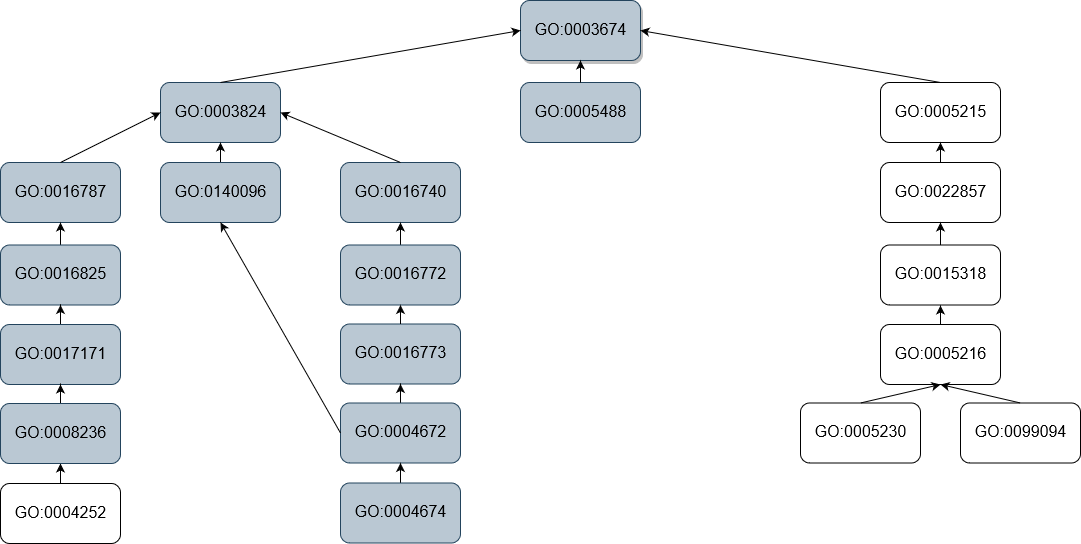
\includegraphics[width=\textwidth]{Figures/LRo.png}
	\caption{Prikaz podgrafa ontologije koji sadrži funkcije iz tabele \ref{tab: lrF1}}
	\label{fig:lr_ontology}
\end{figure}

\begin{table}[h]
	\centering
	\begin{tabular}{|c|c|c|c|c|c|c|c|c|}
		\hline
		Funkcija & F1 & Acc & Pre & Rec & AUC & Nivo & Br. p. & Pr. p. \\
		\hline
		GO:0004672 & 0.81 & 0.978 & 0.84 & 0.78 & 0.88 & 3 & 1257 & 6.0\% \\
		\hline
		GO:0030594 & 0.79 & 0.999 & 0.85 & 0.73 & 0.87 & 3 & 86 & 0.4\% \\
		\hline
		GO:0004930 & 0.78 & 0.992 & 0.73 & 0.84 & 0.92 & 4 & 312 & 1.5\% \\
		\hline
		GO:0005488 & 0.78 & 0.696 & 0.81 & 0.75 & 0.65 & 1 & 15092 & 72.3\% \\
		\hline
		GO:0016773 & 0.76 & 0.97 & 0.81 & 0.72 & 0.85 & 4 & 1377 & 6.6\% \\
		\hline
		GO:0004674 & 0.75 & 0.981 & 0.67 & 0.86 & 0.92 & 4 & 776 & 3.7\% \\
		\hline
		GO:0016301 & 0.75 & 0.967 & 0.82 & 0.68 & 0.84 & 4 & 1452 & 7.0\% \\
		\hline
		GO:0003824 & 0.72 & 0.786 & 0.71 & 0.74 & 0.78 & 1 & 7843 & 37.6\% \\
		\hline
		GO:0019199 & 0.72 & 0.998 & 0.74 & 0.7 & 0.85 & 4 & 78 & 0.4\% \\
		\hline
		GO:0017171 & 0.71 & 0.991 & 0.65 & 0.78 & 0.89 & 4 & 354 & 1.7\% \\
		\hline
		GO:0016825 & 0.71 & 0.992 & 0.75 & 0.67 & 0.83 & 3 & 354 & 1.7\% \\
		\hline
		GO:0008236 & 0.7 & 0.991 & 0.64 & 0.76 & 0.88 & 5 & 349 & 1.7\% \\
		\hline
		GO:0016772 & 0.67 & 0.951 & 0.73 & 0.62 & 0.8 & 3 & 1609 & 7.7\% \\
		\hline
		GO:0004888 & 0.64 & 0.98 & 0.68 & 0.6 & 0.8 & 3 & 626 & 3.0\% \\
		\hline
		GO:0038023 & 0.63 & 0.971 & 0.69 & 0.57 & 0.78 & 2 & 909 & 4.4\% \\
		\hline
		GO:0060089 & 0.62 & 0.967 & 0.66 & 0.59 & 0.79 & 1 & 976 & 4.7\% \\
		\hline
		GO:0140096 & 0.59 & 0.883 & 0.66 & 0.54 & 0.75 & 2 & 3337 & 16.0\% \\
		\hline
		GO:1901363 & 0.57 & 0.728 & 0.54 & 0.61 & 0.69 & 2 & 6236 & 29.9\% \\
		\hline
		GO:0016740 & 0.55 & 0.873 & 0.59 & 0.51 & 0.72 & 2 & 3069 & 14.7\% \\
		\hline
		GO:0016787 & 0.48 & 0.842 & 0.48 & 0.49 & 0.7 & 2 & 3202 & 15.3\% \\
		\hline
	\end{tabular}
	\caption{Prikaz mera kvaliteta za pojedina\v cne klasifikatore metode potpornih vektora za 20 \v cvorova sa najboljom $f1$-merom}
	\label{tab: svmF1}
\end{table}


~\\
~\\

Najbolji modeli metode potpornih vektora pokazuju slično ponašanje kao modeli logističke regresije.

~\\

\begin{figure}[H]
	\centering
	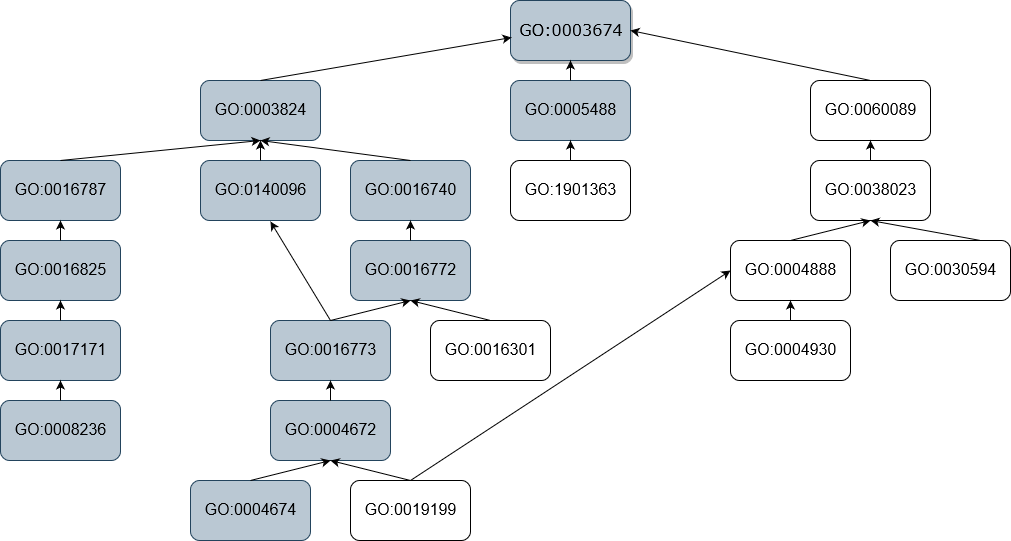
\includegraphics[width=\textwidth]{Figures/SVMo.png}
	\caption{Prikaz podgrafa ontologije koji sadrži funkcije iz tabele \ref{tab: svmF1}}
	\label{fig:svm_ontology}
\end{figure}

\newpage

Prikazani podgrafi sadrže zajedničke čvorove odnosno, sva tri prediktora su za nekoliko istih funkcija dali najbolje rezultate. Nazivi ovih funckija navedeni su u tabeli \ref{tab: commonNames}. Poređenje mera kvaliteta klasifikatora ovih funkcija prikazano je u tabeli \ref{tab: commonScores}, a na slikama su zajednički čvorovi označeni sivom bojom.

~\\

\begin{table}[H]
	\centering
	\begin{tabular}{|c|l|}
		\hline
		Oznaka funkcije & Naziv funkcije \\
		\hline
		GO:0003674 & molecular\_function\\
		\hline
		GO:0003824 & catalytic activity\\
		\hline
		GO:0005488 & binding\\
		\hline
		GO:0016787 & hydrolase activity\\
		\hline
		GO:0140096 & catalytic activity, acting on a protein\\
		\hline
		GO:0016740 & transferase activity\\
		\hline
		GO:0016825 & hydrolase activity, acting on acid phosphorus-nitrogen bonds \\
		\hline
		GO:0016772 & transferase activity, transferring phosphorus-containing groups\\
		\hline
		GO:0017171 & serine hydrolase activity \\
		\hline
		GO:0016773 & phosphotransferase activity, alcohol group as acceptor \\
		\hline
		GO:0008236 & serine-type peptidase activity \\
		\hline
		GO:0004672 & protein kinase activity \\
		\hline
		GO:0004674 & protein serine/threonine kinase activity \\
		\hline
	\end{tabular}
	\caption{Oznake i nazivi funkcija za zajedničke čvorove podgrafa sa slika \ref{fig:rf_ontology}, \ref{fig:lr_ontology} i \ref{fig:svm_ontology}} 
	\label{tab: commonNames}
\end{table}


~\\

Modeli metode slučajnih šuma za iste funkcije daju nešto slabiju $f1$-meru u poređenju sa ostalim metodama, ali zato je preciznost skoro svih modela veća u odnosu na modele drugih metoda. Tačnost svih modela su prilično bliske, dok se prema odzivu najviše ističu modeli linearne regresije. Površina ispod ROC krive je slična za modele logističke regresije i modela potpornih vektora, a slučajne šume su dale nešto slabije rezultate.



\begin{landscape}
\begin{table}[H]
	\centering
	\begin{tabular}{V{3.5}cV{3.5}c|c|cV{3.5}c|c|cV{3.5}c|c|cV{3.5}c|c|cV{3.5}c|c|cV{3.5}}
		\hlineB{3.5}
		\multirow{3}{*}{Oznaka funkcije} & \multicolumn{3}{cV{3.5}}{\multirow{2}{*}{F1-mera}} & \multicolumn{3}{cV{3.5}}{\multirow{2}{*}{Ta\v cnost}}  & \multicolumn{3}{cV{3.5}}{\multirow{2}{*}{Preciznost}} & \multicolumn{3}{cV{3.5}}{\multirow{2}{*}{Odziv}}  & \multicolumn{3}{cV{3.5}}{Povr\v sina ispod} \\
		& \multicolumn{3}{cV{3.5}}{} & \multicolumn{3}{cV{3.5}}{} & \multicolumn{3}{cV{3.5}}{} & \multicolumn{3}{cV{3.5}}{} & \multicolumn{3}{cV{3.5}}{ROC krive} \\
		\cline{2-16}
		& LR & RF & SVM & LR & RF & SVM & LR & RF & SVM & LR & RF & SVM & LR & RF & SVM \\
		\hlineB{3.5}
		GO:0003824 & 0.71 & 0.52 & \textbf{0.72} &0.76 & 0.74 & \textbf{0.79} &0.65 & \textbf{0.84} & 0.71 & \textbf{0.77} & 0.37 & 0.74 &0.76 & 0.67 & \textbf{0.78}\\
		\hline
		GO:0005488 & 0.76 & \textbf{0.84} & 0.78 & 0.67 & \textbf{0.73} & 0.7 & 0.8 & 0.74 & \textbf{0.81} & 0.73 & \textbf{0.97} & 0.75 & 0.63 & 0.54 & \textbf{0.65}\\
		\hline
		GO:0016787 & 0.46 & 0.23 & \textbf{0.48} & 0.81 & \textbf{0.86} & 0.84 & 0.4 & \textbf{0.77} & 0.48 & \textbf{0.55} & 0.13 & 0.49 & \textbf{0.7} & 0.56 & \textbf{0.7}\\
		\hline
		GO:0140096 & \textbf{0.59} & 0.42 & \textbf{0.59} & 0.86 & \textbf{0.88} & \textbf{0.88} &0.54 & \textbf{0.89} & 0.66 & \textbf{0.65} & 0.27 & 0.54 & \textbf{0.78} & 0.63 & 0.75\\
		\hline
		GO:0016740 & 0.53 & 0.36 & \textbf{0.55} & 0.84 & \textbf{0.88} & 0.87 & 0.49 & \textbf{0.92} & 0.59 & \textbf{0.58} & 0.23 & 0.51 & \textbf{0.74} & 0.61 & 0.72\\
		\hline
		GO:0016825 & 0.69 & 0.56 & \textbf{0.71} & \textbf{0.99} & \textbf{0.99} & \textbf{0.99} & 0.68 & \textbf{0.91} & 0.75 & \textbf{0.71} & 0.4 & 0.67 & \textbf{0.85} & 0.7 & 0.83\\
		\hline
		GO:0016772 & \textbf{0.67} & 0.46 & \textbf{0.67} & \textbf{0.95} & 0.94 & \textbf{0.95} & 0.69 & \textbf{0.96} & 0.73 & \textbf{0.64} & 0.31 & 0.62 & \textbf{0.81} & 0.65 & 0.8\\
		\hline
		GO:0017171 & 0.69 & 0.57 & \textbf{0.71} & \textbf{0.99} & \textbf{0.99} & \textbf{0.99} & 0.69 & \textbf{0.91} & 0.65 & 0.68 & 0.42 & \textbf{0.78} & 0.84 & 0.71 & \textbf{0.89}\\
		\hline
		GO:0016773 & \textbf{0.77} & 0.51 & 0.76 & \textbf{0.97} & 0.96 & \textbf{0.97} & 0.78 & \textbf{0.94} & 0.81 & \textbf{0.75} & 0.35 & 0.72 & \textbf{0.87} & 0.67 & 0.85\\
		\hline
		GO:0008236 & \textbf{0.7} & 0.54 & \textbf{0.7} & \textbf{0.99} & \textbf{0.99} & \textbf{0.99} & 0.71 & \textbf{0.93} & 0.64 & 0.69 & 0.38 & \textbf{0.76} & 0.84 & 0.69 & \textbf{0.88}\\
		\hline
		GO:0004672 & \textbf{0.82} & 0.53 & 0.81 & \textbf{0.98} & 0.96 & \textbf{0.98} & 0.82 & \textbf{0.92} & 0.84 & \textbf{0.81} & 0.37 & 0.78 & \textbf{0.9} & 0.69 & 0.88\\
		\hline
		GO:0004674 & 0.74 & 0.44 & \textbf{0.75} & \textbf{0.98} & 0.97 & \textbf{0.98} & 0.65 & \textbf{0.8} & 0.67 & \textbf{0.87} & 0.3 & 0.86 & \textbf{0.93} & 0.65 & 0.92\\
		\hlineB{3.5}
	\end{tabular}
	\caption{Pore\dj enje mera kvaliteta za zajedni\v cke \v cvorove podgrafa sa slika \ref{fig:rf_ontology}, \ref{fig:lr_ontology} i \ref{fig:svm_ontology}} 
	\label{tab: commonScores}
	\end{table}
	
\end{landscape}

Predikotri su dodatno testirani na \textit{benchmark} skupu proteina koji je korišćen u okviru CAFA3 takmičenja \cite{biofCafa}. Skup sadrži 453 proteina različitih organizama. Izračunata je prosečna vrednost $f_1$-mera za svaki prediktor, a dobijeni rezultati su dodatno upoređeni sa rezultatima učesnika takmičenja \cite{cafa}. 

Prediktor za metodu slučajnih šuma dao je najbolji rezultat od tri prediktora, čime je među učesnicima ovog takmičenja zauzeo 85. mesto među 136 tačkmičara. Poređenje sva tri prediktora sa svim učesnicima prikazano je na slici \ref{fig:cafa}.


\begin{figure}[H]
	\centering
	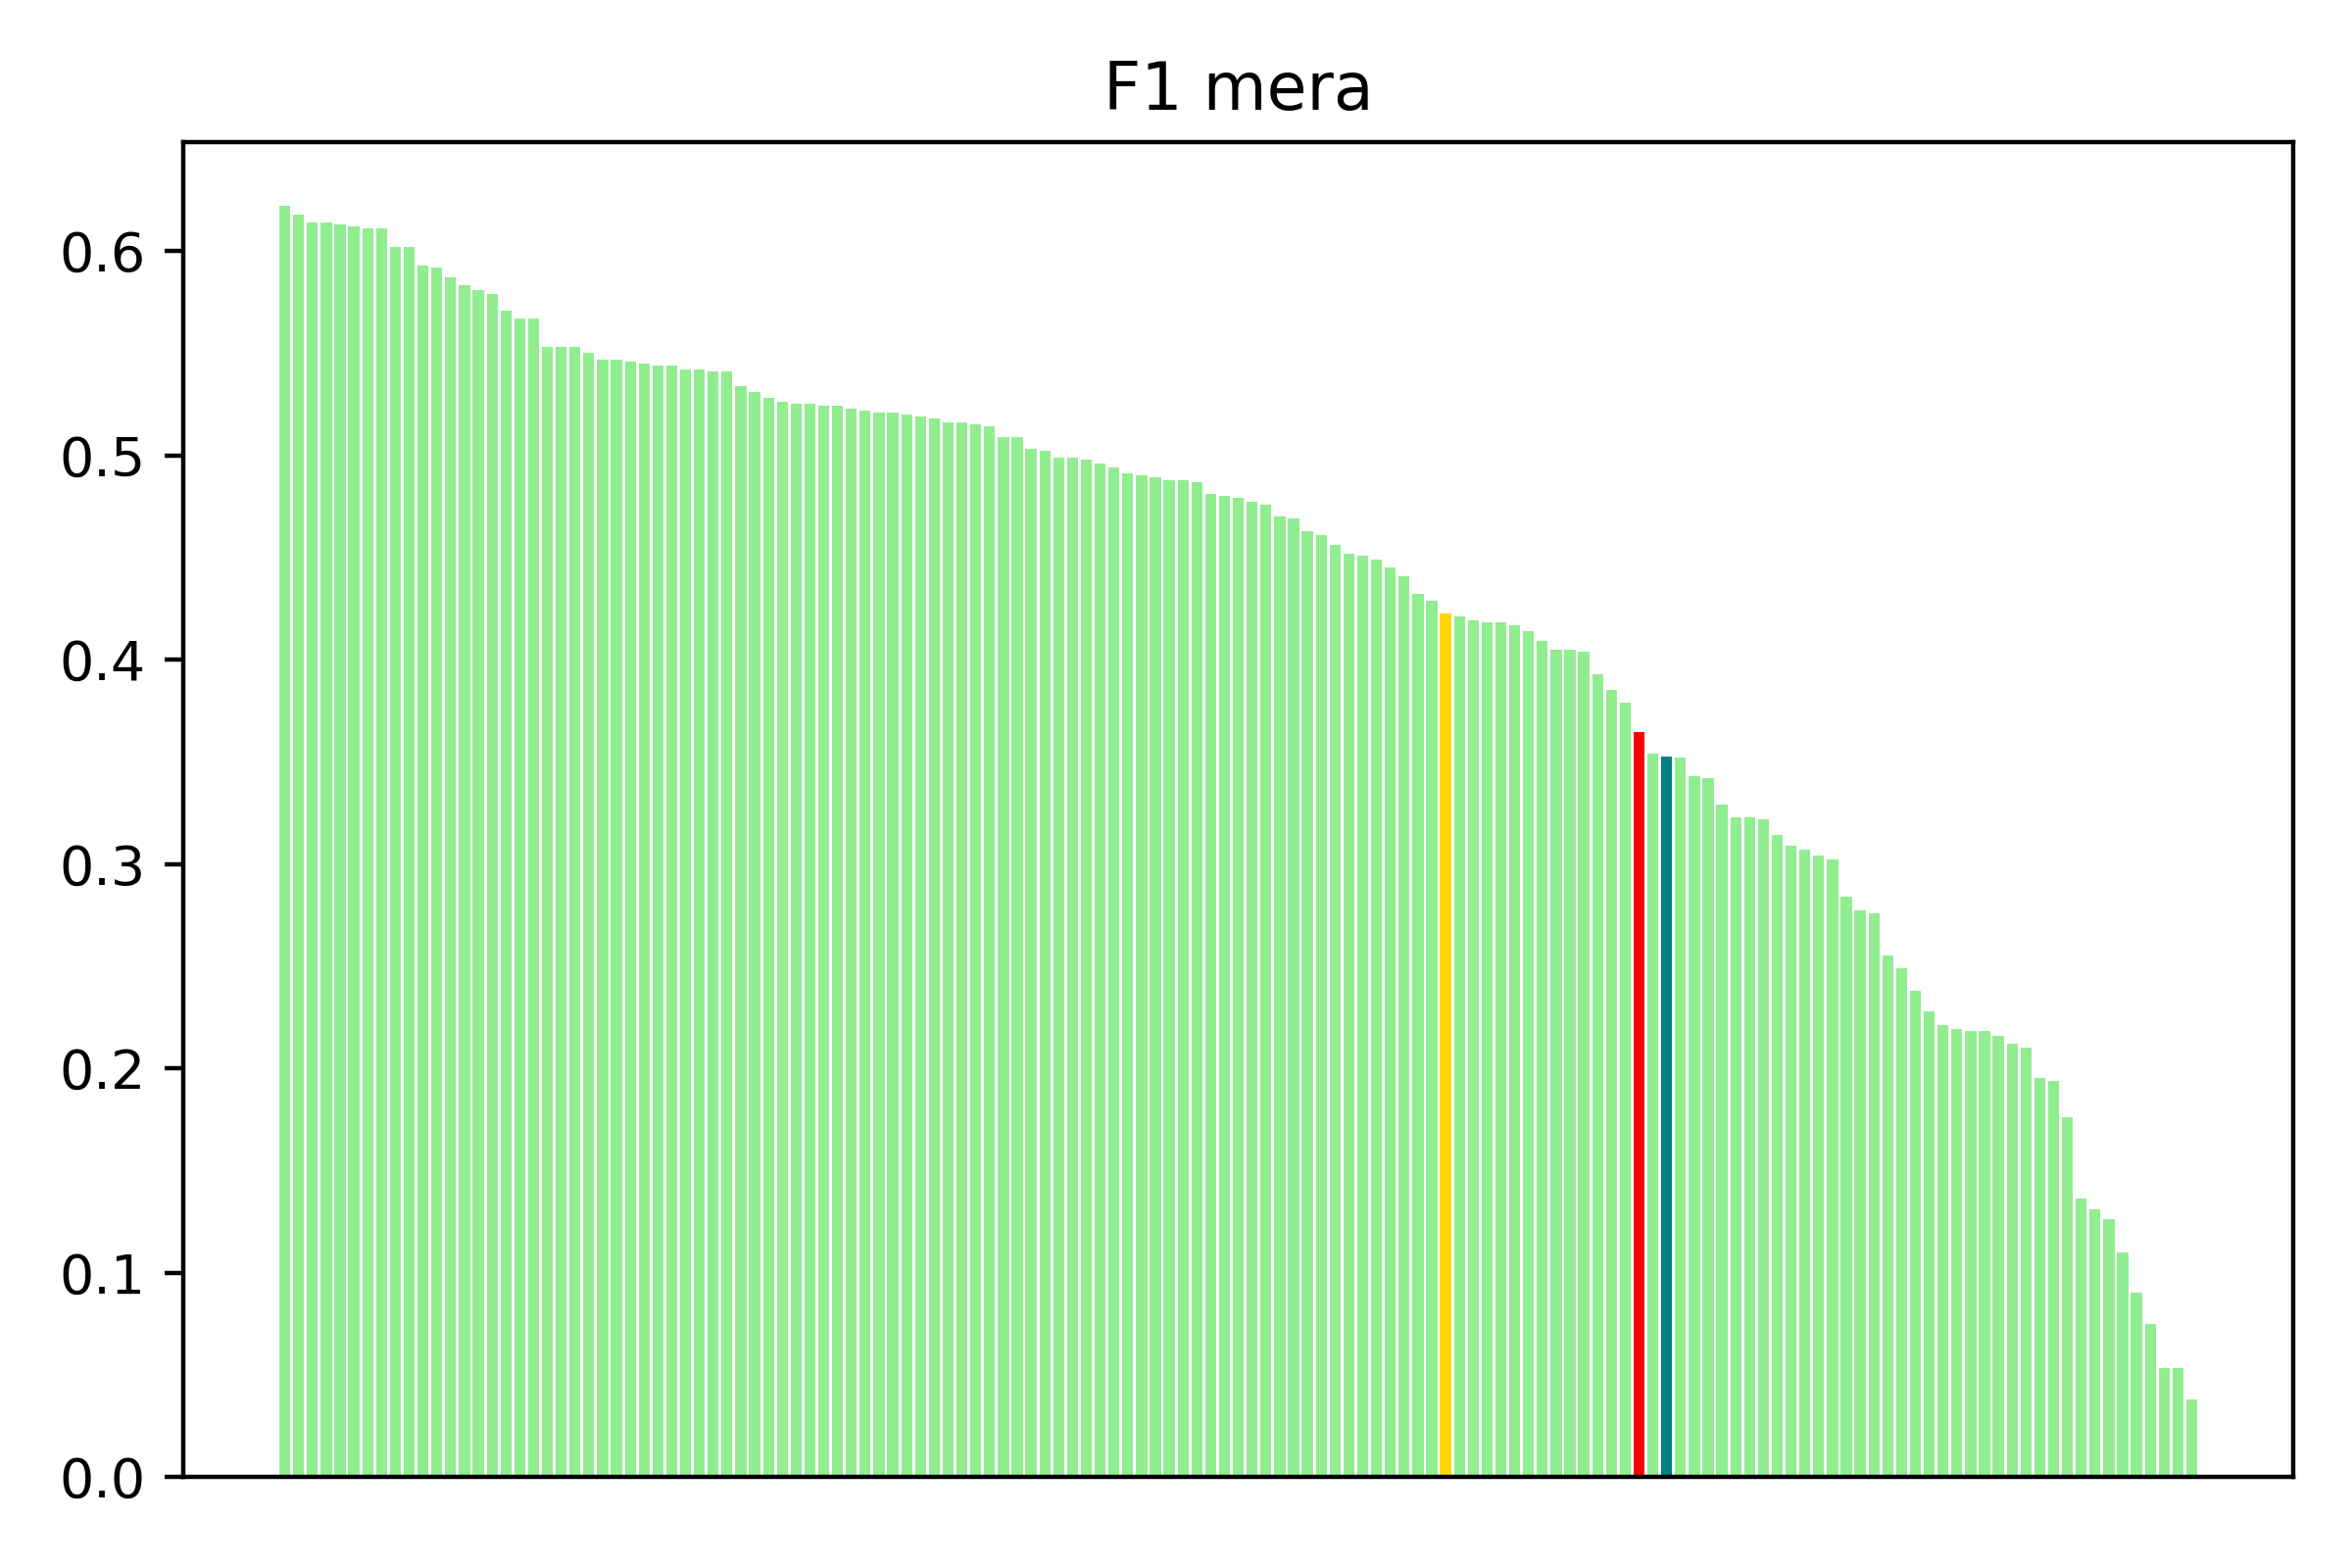
\includegraphics[width=\textwidth]{Figures/cafa_poredjenje.png}
	\caption{Poređenje $f_1$-mera tri prediktora sa rezultatima učesnika  CAFA3 takmičenja. Crvenom bojom označen je prediktor linearne regresije, žutom prediktor slučajnih šuma, plavom prediktor metode potpornih vektora. Svetlo zelenom bojom prikazani su rezultati postignuti na CAFA3 takmičenju.}
	\label{fig:cafa}
\end{figure}



%\chapter{Zaključak} % Main chapter title
\label{Chapter7}

U ovom radu prikazan je razvoj tri prediktora za predviđanje funkcije proteina. Računarski metodi za određivanje funkcija razvijaju se godinama, ali i dalje nema metoda koji može da odredi funkciju proteina preciznije od eksperimentalnog metoda. Kao što je već pomenuto, eksperimentalno utvrđivanje funkcije proteina je skup i spor proces zbog čega je ovaj problem i dalje aktuelan i od velikog značaja. 


Iako su se obučeni prediktori pokazali bolje od naivnog klasifikatora, nemaju približnu moć predviđanja u poređenju sa aktivnim rezultatima prikazanim na poslednjem CAFA takmičenju, najrelevantnijem takmičenju u ovoj oblasti. Planovi za unapređivanje prediktora obuhvataju:

\begin{itemize}
	\item treniranje pojedinačnih modela i prediktora za svaki od organizama - cilj je utvrditi da li će se prediktori bolje ponašati za određeni organizam ukoliko se obučavaju na proteinima koji potiču isključivo iz tog organizma,
	
	\item povećanje trening skupa - zbog malog broja pozitivnih instanci, za određene funkcije nije pravljen klasifikator,
	
	\item promenu ulaznih podataka - ideja je povećati vrednost parametra $k$ koji određuje dužinu podniski, a samim tim i niza kojim se predstavlja protein,
	
	\item korišćenje raznovrsnijih metoda binarne klasifikacije - na primer, neuronskih mreža.
\end{itemize}




%----------------------------------------------------------------------------------------
%	THESIS CONTENT - APPENDICES
%----------------------------------------------------------------------------------------

\appendix % Cue to tell LaTeX that the following "chapters" are Appendices

% Include the appendices of the thesis as separate files from the Appendices folder
% Uncomment the lines as you write the Appendices

% % Appendix A

\chapter{Frequently Asked Questions} % Main appendix title

\label{AppendixA} % For referencing this appendix elsewhere, use \ref{AppendixA}

\section{How do I change the colors of links?}

The color of links can be changed to your liking using:

{\small\verb!\hypersetup{urlcolor=red}!}, or

{\small\verb!\hypersetup{citecolor=green}!}, or

{\small\verb!\hypersetup{allcolor=blue}!}.

\noindent If you want to completely hide the links, you can use:

{\small\verb!\hypersetup{allcolors=.}!}, or even better: 

{\small\verb!\hypersetup{hidelinks}!}.

\noindent If you want to have obvious links in the PDF but not the printed text, use:

{\small\verb!\hypersetup{colorlinks=false}!}.

%\include{Appendices/AppendixB}
%\include{Appendices/AppendixC}

%----------------------------------------------------------------------------------------
%	BIBLIOGRAPHY
%----------------------------------------------------------------------------------------
\renewcommand{\bibname}{Bibliografija}
\printbibliography[heading=bibintoc]

%----------------------------------------------------------------------------------------

\end{document}  
